\documentclass[11pt, twoside, a4paper]{report}

% Language
\usepackage[T1]{fontenc}  % ensure that type 1 fonts (vector-based)

% General
\usepackage{fancyhdr}
\RequirePackage[nottoc]{tocbibind} % include bibliography in table of contents
\usepackage{parskip} % manages the two lengths \parskip and \parindent
\usepackage{placeins} % preventing floats from floating past a \FloatBarrier
\usepackage{caption} % enables caption customization
\usepackage[all]{nowidow} % removes orphans and widows
\usepackage{geometry} % document layout.
\usepackage{titling} % user-friendly access of title, author, etc. 

% Font
\usepackage{lmodern} % use improved fonts compared to the standard latex fonts
\usepackage{anyfontsize} % for proper scaling of font sizes 
\usepackage{xcolor} % for coloured text with command \color{<color>}{<text>}
\usepackage{xspace} % define commands that appear not to eat spaces
\usepackage[utf8]{inputenc} % german umlaut (ö, ä, ü)

% Graphics
\usepackage{graphicx} % include graphics
\usepackage{float} % adds feature to place floats where defined via h! or H!
\usepackage{pgfplots} % adds native plotting features to LaTeX

% Math Symbols
\usepackage{amsmath} % most of the mathematical features of AMS-TEX
\usepackage{amssymb} % provides an extended symbol collection and loads amsfonts
\usepackage{amsthm} % helps to define theorem-like structures
\usepackage{mathtools} % fixes various deficiencies of amsmath and standard LATEX
\usepackage{mathabx} % provides even more mathematical symbols
\usepackage{commath} % for nice derivative operators

% Text Symbols
\usepackage{acronym}
\usepackage{textcomp} % provides an extensive list of text symbols
\usepackage{xfrac} % provides the command \sfrac to print nice d/n fractions

% Units
\usepackage{units} % bundle for typesetting physical units and nice fractions

% Tables & Images
\usepackage{multirow} % construction for table cells that span more than one row
\usepackage{array} % extends options for tabular environment
\usepackage{booktabs} % enhances quality of tables and provides extra commands

% Environments
\usepackage[chapter]{algorithm} % for floating algorithm environment
\usepackage[noend]{algpseudocode} % for pseudocode environment
\usepackage{fancyvrb} % allows to indent the verbatim environment
\usepackage{enumitem} % allows to customize lists such as itemize and enumerate
\usepackage{ragged2e} % allows setting ragged text which is easy to configure
\usepackage{csquotes} % advanced facilities for inline and display quotations
\usepackage{listings} % advanced typesetting of source code
\usepackage{setspace} % line stretching in environment

% Graphics.
\usepackage{tikz} % control flow and other diagrams
\usepackage{pgfplots} % more plotting (coordinate systems)
\usepackage{pgf-pie}

\pgfplotsset{compat=1.11}
\usepackage{tkz-euclide}
\usepgfplotslibrary{fillbetween}
\usetikzlibrary{shapes, arrows}

\tikzset{velocity/.style={->, densely dashed, thick, draw=black}}

% Internet addresses and interactive links
\usepackage[hyphens]{url}
\usepackage[colorlinks=true, linkcolor=black, urlcolor=blue, citecolor=black]{hyperref}

% Problem and corollary definition. 
\newtheorem{problem}{Problem}
\newtheorem{theorem}{Theorem}[section]
\newtheorem{corollary}{Corollary}[section]

% Document info _______________________________________________________
\title{Mantrap}
\author{Simon Schaefer}

\def \project{mantrap}
\def \ethid{14-943-799}
\def \email{sischaef@student.ethz.ch}
\def \semester{6}
\def \phdA{Karen Leung}
\def \phdB{Boris Ivanovic}
\def \supervisoreth{Prof. Emilio Frazzoli}
\def \supervisorstanford{Prof. Marco Pavone}

\def \imgwidth{0.7\textwidth}
\def \algorithmstretch{1.2}

\def \x{\boldsymbol{x}}
\def \dx{\boldsymbol{\dot{x}}}
\def \ddx{\boldsymbol{\ddot{x}}}
\def \u{\boldsymbol{u}}

\def \xped[#1]{\boldsymbol{\tilde{x}^{#1}}}
\def \dxped[#1]{\boldsymbol{\dot{\tilde{x}}^{#1}}}
\def \ddxped[#1]{\boldsymbol{\ddot{\tilde{x}}^{#1}}}
\def \uped[#1]{\boldsymbol{\tilde{u}^{#1}}}

\def \muped[#1]{\boldsymbol{\tilde{\mu}^{#1}}}
\def \sigmaped[#1]{\boldsymbol{\tilde{\Sigma}^{#1}}}
\def \piped[#1]{\boldsymbol{\tilde{\pi}^{#1}}}

\def \xpedwo[#1]{\boldsymbol{\tilde{\chi}^{#1}}}
\def \dxpedwo[#1]{\boldsymbol{\dot{\tilde{\chi}}^{#1}}}
\def \ddxpedwo[#1]{\boldsymbol{\ddot{\tilde{\chi}}^{#1}}}

\def \dist[#1]{\boldsymbol{\tilde{\psi}^{#1}}}
\def \distwo[#1]{\boldsymbol{\tilde{\Psi}^{#1}}}
\def \distmodel[#1]{\boldsymbol{\tilde{\Gamma}^{#1}}}
\def \distmodeldet[#1]{\boldsymbol{\tilde{\gamma}^{#1}}}

\def \d{\boldsymbol{x}_{rel}}
\def \xrel{\boldsymbol{x}_{rel}}
\def \Vrel{V}
\def \frel{f_{rel}}

\def \xset{\mathcal{X}}
\def \uset{\mathcal{U}}
\def \upedset{\mathcal{\tilde{U}}}

\def \dt{\delta t}
\def \f{f}
\def \pstate[#1]{\boldsymbol{\rho}^{#1}}  % particles (based prediction)
\def \pparam[#1]{\boldsymbol{\theta}^{#1}}

\def \stepssolution{N}
\def \goal{\boldsymbol{g}}


% Page format _________________________________________________________
\frenchspacing % makes the sentence spacing single spaced
\setlength{\parindent}{0em}                 % Disable par-indent
\setlength{\headheight}{14pt}				% Correcting too small head height
\rhead[\nouppercase{\rightmark}]{\thepage}  % Special headings
\lhead[\thepage]{\nouppercase{\leftmark}}   % Special headings
\cfoot{}                                    % Special headings

\setcounter{tocdepth}{2} % Table of contents contain only chapters and sections
\captionsetup[table]{skip=10pt} % Increase space between tables and caption

% Document ____________________________________________________________
\begin{document}
\begin{titlepage}

\pagestyle{empty}
\newgeometry{hmargin=2cm, vmargin=2.5cm}
\begin{center}

% Institute and ETH logos

\includegraphics[height=1.6cm]{logos/eth_logo}
\hfill

\includegraphics[height=1.6cm]{logos/idsc_logo}

% Author name(s)
\vspace*{2cm}
{\large \theauthor}
\vspace{2.5cm}

% Title of work
\begin{minipage}{15cm}
\centering
\bfseries \Huge {\thetitle} 
\\\vspace*{1cm}\Large {Minimally interfering Interactive Risk-aware Planning for multimodal and time-evolving obstacle behavior}
\end{minipage}
\vspace*{4cm}


% Affiliation
{\large \textbf{Master Thesis}} \\[3ex]
Institute for Dynamic Systems and Control\\
Swiss Federal Institute of Technology (ETH) Zurich\\

% Supervisors
\vspace{2cm}
\textbf{Supervision} \\[1.5ex]
\phdA \\
\phdB \\ 
\supervisorstanford \\ 
\supervisoreth

% Date
\vfill
\today

% End of title page
\end{center}

\cleardoublepage % required. Otherwise Abstract appears directly on second page
\end{titlepage}


% Pre-Document ________________________________________________________
\pagenumbering{roman}	% Begin roman page numbering (i,ii,...) j

\cleardoublepage
\chapter*{Preface}
This thesis was carried out at the \ac{ASL} at Stanford University. First of all, I want to thank Prof. Marco Pavone for hosting me in his laboratory and supervising this work. Each discussion was insightful and helped shaping this project. I also want to thank Prof. Emilio Frazzoli for co-supervising this thesis and advising me during my studies at \ac{ETH}.
\newline
Working at \ac{ASL} was a very enriching experience and I want to thank all the members of the lab for welcoming me in this unique environment. I am deeply grateful to Karen Leung and Boris Ivanovic for their constant advice, for sharing their knowledge and experience about optimization, trajectory optimization and other related subjects.
\newline
When I arrived at Stanford, the field of (trajectory) optimization was obscure to me. I am very thankful for the help and for the fruitful discussions with several lab members as well as lab visitors; Tim Salzmann for the many discussions about machine learning, Riccardo Bonalli and Matteo Zallio for their advice and the insightful discussions over lunch, Robert Dyro for his support in efficient PyTorch programming, Jan Carius for his introduction to trajectory optimization, Jan Schiliger for his knowledge about control theory,  Thomas Lew and Layla Martin for their advice in (general) optimization techniques and Lina Fang for proof-reading my work. I will always be grateful to my family which has always been supportive throughout my life, encouraged me during my studies and greatly supported me throughout my thesis in this difficult times. Finally, I am grateful to the \ac{ETH} Excellence Scholarship and Opportunities Program as well as the Werner Siemens Foundation for financially supporting my stay at Stanford.

\cleardoublepage

%% Table of Contents ___________________________________________________
\tableofcontents

\cleardoublepage
\chapter*{Abstract}
\addcontentsline{toc}{chapter}{Abstract}

Abstract is missing

\vspace{1cm}
\textbf{Keywords}: 

\cleardoublepage
\chapter*{Nomenclature}
\addcontentsline{toc}{chapter}{Nomenclature}

\section*{Symbols}
\begin{tabbing}
\hspace*{1.6cm} \= \hspace*{8cm} \= \kill
$\mathbb{R}^n$ \> set of real column vectors of length n \\[0.5ex]
$\mathbb{R}^{m \times n}$ \> set of real m by n matrices \\[0.5ex]
$\mathbf{0}_{m \times n}$ \> n by m zero matrix \\[0.5ex]
$\mathbf{I}_n$ \> identity matrix of dimension n \\[0.5ex]
$\x$ \> state of robot \\[0.5ex]
$\u$ \> control input of robot \\[0.5ex]
$\xped[k]$ \> state of pedestrian k \\[0.5ex]
$\uped[k]$ \> control input of pedestrian k \\[0.5ex]
$\muped[k]$ \> mean of state $\xped[k]$ \\[0.5ex]
$\sigmaped[k]$ \> variance of state $\xped[k]$ \\[0.5ex]
$\piped[k]$ \> mode importance of state $\xped[k]$ \\[0.5ex]
$\goal$ \> goal state \\[0.5ex]
$\xset$ \> set of feasible states \\[0.5ex]
$\xset_0$ \> set of initial states \\[0.5ex]
$\xset_f$ \> set of terminal/goal states \\[0.5ex]
$\xset_{rel}$ \> Hamilton-Jacobi reachability joint states set \\[0.5ex]
$\xset_{avoid}$ \> Hamilton-Jacobi reachability avoid set \\[0.5ex]
$\uset$ \> set of feasible controls of robot \\[0.5ex]
$\upedset$ \> set of feasible controls of pedestrian \\[0.5ex]
$t_0$ \> initial time of optimization [s] \\[0.5ex]
$t_f$ \> final time of optimization [s] \\[0.5ex]
$T$ \> optimization horizon in discrete steps \\[0.5ex]
$\Delta t$ \> discretization time of the dynamics [$s$] \\[0.5ex]
$\dt$ \> time-step of Runge-Kutta integration method [$s$] \\[0.5ex]
$K$ \> number of pedestrians \\[0.5ex]
$k$ \> pedestrian index \\[0.5ex]
$L$ \> number of pedestrian prediction modes \\[0.5ex]
$l$ \> prediction mode index \\[0.5ex]
$n$ \> dimension of state $\x$ \\[0.5ex]
$m$ \> dimension of control input $\u$ \\[0.5ex]
$\stepssolution$ \> number of solution time-steps from initial to target state \\[0.5ex]
$\f(\cdot)$ \> system dynamics of robot \\[0.5ex]
$\frel(\cdot)$ \> joint robot-pedestrian system dynamics \\[0.5ex]
$J(\cdot)$ \> cost function \\[0.5ex]
$l(\cdot)$ \> step cost function \\[0.5ex]
$l_f(\cdot)$ \> final cost function \\[0.5ex]
$\Vrel(\cdot)$ \> Hamilton-Jacobi reachability value function \\[0.5ex]
$\mathcal{N}(\cdot)$ \> normal probability distribution \\[0.5ex]
\end{tabbing}

\section*{Operators}
\begin{tabbing}
\hspace*{1.6cm} \= \hspace*{8cm} \= \kill
$\mathbb{E}_Y[\cdot]$ \> expectation operator with respect to $Y$ \\[0.5ex]
$\mathrm{Var}_Y[\cdot]$ \> variance operator with respect to $Y$ \\[0.5ex]
$\max$ \> maximum operator \\[0.5ex]
$\min$ \> minimum operator \\[0.5ex]
$||\cdot||_1$ \> L1 norm (absolute value) \\[0.5ex]
$||\cdot||_2$ \> L2 norm (euclidean distance) \\[0.5ex]
$||\cdot||_{\infty}$ \> L-infinity norm (maximal value) \\[0.5ex]
\end{tabbing}

\section*{Indexing}
\begin{tabbing}
\hspace*{1.6cm} \= \hspace*{8cm} \= \kill
$\mathbf{a}_i$ \> element $i$ of vector $\mathbf{a}$ \\[0.5ex]
$\mathbf{A}_{ij}$ \> element in row $i$ and column $j$ of matrix $\mathbf{A}$ \\[0.5ex]
\end{tabbing}


\section*{Acronyms and Abbreviations}
\begin{acronym}[Bash]
\acro{ETH}{Eidgenössische Technische Hochschule}
\acro{IDSC}{Institute of Dynamical Systems and Control at ETH Zürich}
\acro{ASL}{Autonomous Systems Lab at Stanford University}
\acro{NLP}{Non-Linear Program}
\acro{IPOPT}{Interior Point Optimiser \cite{Wachter2006}}
\acro{GuSTO}{Guaranteed Sequential Trajectory optimization \cite{Bonalli2019}}
\acro{SQP}{Sequential Quadratic Programs}
\acro{IPM}{Interior Point Methods}
\acro{GMM}{Gaussian Mixture Model}
\acro{PDF}{Probability Density Function}
\acro{ELBO}{Evidence-based Lower Bound}
\acro{ORCA}{Optimal Reciprocal Collision Avoidance}
\acro{RRT}{Rapidly-exploring Random Trees}
\acro{MCTS}{Monte-Carlo Tree Search}
\acro{SGAN}{Socially Generative Adversarial Network}
\acro{HJR}{Hamilton-Jacobi Reachability}
\acro{ODE}{Ordinary Differential Equation}
\acro{PP}{Probabilistic Programming}
\acro{IRL}{Inverse Reinforcement Learning} 
\acro{LSTM}{Long Short-Term Memory}
\acro{GAN}{Generative Adversarial Network}
\acro{VAE}{Variational Auto-Encoder}
\acro{POMDP}{Partial Observable Markov Decision Process}
\acro{GFW}{Goal Focussed Warm-Start}
\acro{SCW}{Safety Concerned Warm-Start}
\acro{PCBW}{Pre-Computation-Based Warm-Start}
\acro{SPMW}{Simplified-Prediction-Model Warm-Start}
\acro{RCE}{Robot Control Effort}
\acro{MSD}{Minimal Separation Distance}
\acro{RTD}{Robot Trajectory Directness}
\acro{ETT}{Extra Travel Time}
\acro{MPE}{Mean Pedestrian Effort}
\acro{TGD}{Terminal Goal Distance}
\acro{MSI}{Mean Solving Iterations}
\acro{M95OD}{Mean 95 \% Objective Decay}
\acro{MSR}{Mean Solving Runtime}
\end{acronym}

 \cleardoublepage

% Report ______________________________________________________________
\pagestyle{fancy}       	% Fancy headings
\pagenumbering{arabic} 	% Begin arabic page numbering (1,2,...)

\chapter{Introduction and Motivation}
\label{text:introduction}
Autonomous systems play an increasingly fundamental role in our society. A study of McKinsey in 2017 showed the large effects increasing automatic will have on the economy; one of the key inside of the study is that even as automation causes declines in some occupations, it will change many more, with estimated 60 percent of occupations of which at least 30 percent of constituent work activities will be automated \footnote{\href{https://www.mckinsey.com/~/media/McKinsey/Featured\%20Insights/Future\%20of\%20Organizations/What\%20the\%20future\%20of\%20work\%20will\%20mean\%20for\%20jobs\%20skills\%20and\%20wages/MGI-Jobs-Lost-Jobs-Gained-Report-December-6-2017.ashx}{Jobs lost, Jobs gained: Workforce transitions in a time of automation - McKinsey Global International}}. The International Federation of Robotics, an association of unilateral robotics societies and companies operating in the field, illustrated the rise of service robots in many fields, such as logistics, healthcare or agriculture, in its annual report 2019.\footnote{\href{https://ifr.org/downloads/press2018/IFR\%20World\%20Robotics\%20Presentation\%20-\%2018\%20Sept\%202019.pdf}{Annual Report 2019 - IFR}} Next to the field of fully autonomous robots there also they state an increasing share of collaborative robots, e.g. assisting object retrieval in warehouses or cleaning in hospitals.

\begin{figure}[!ht]
\begin{center}
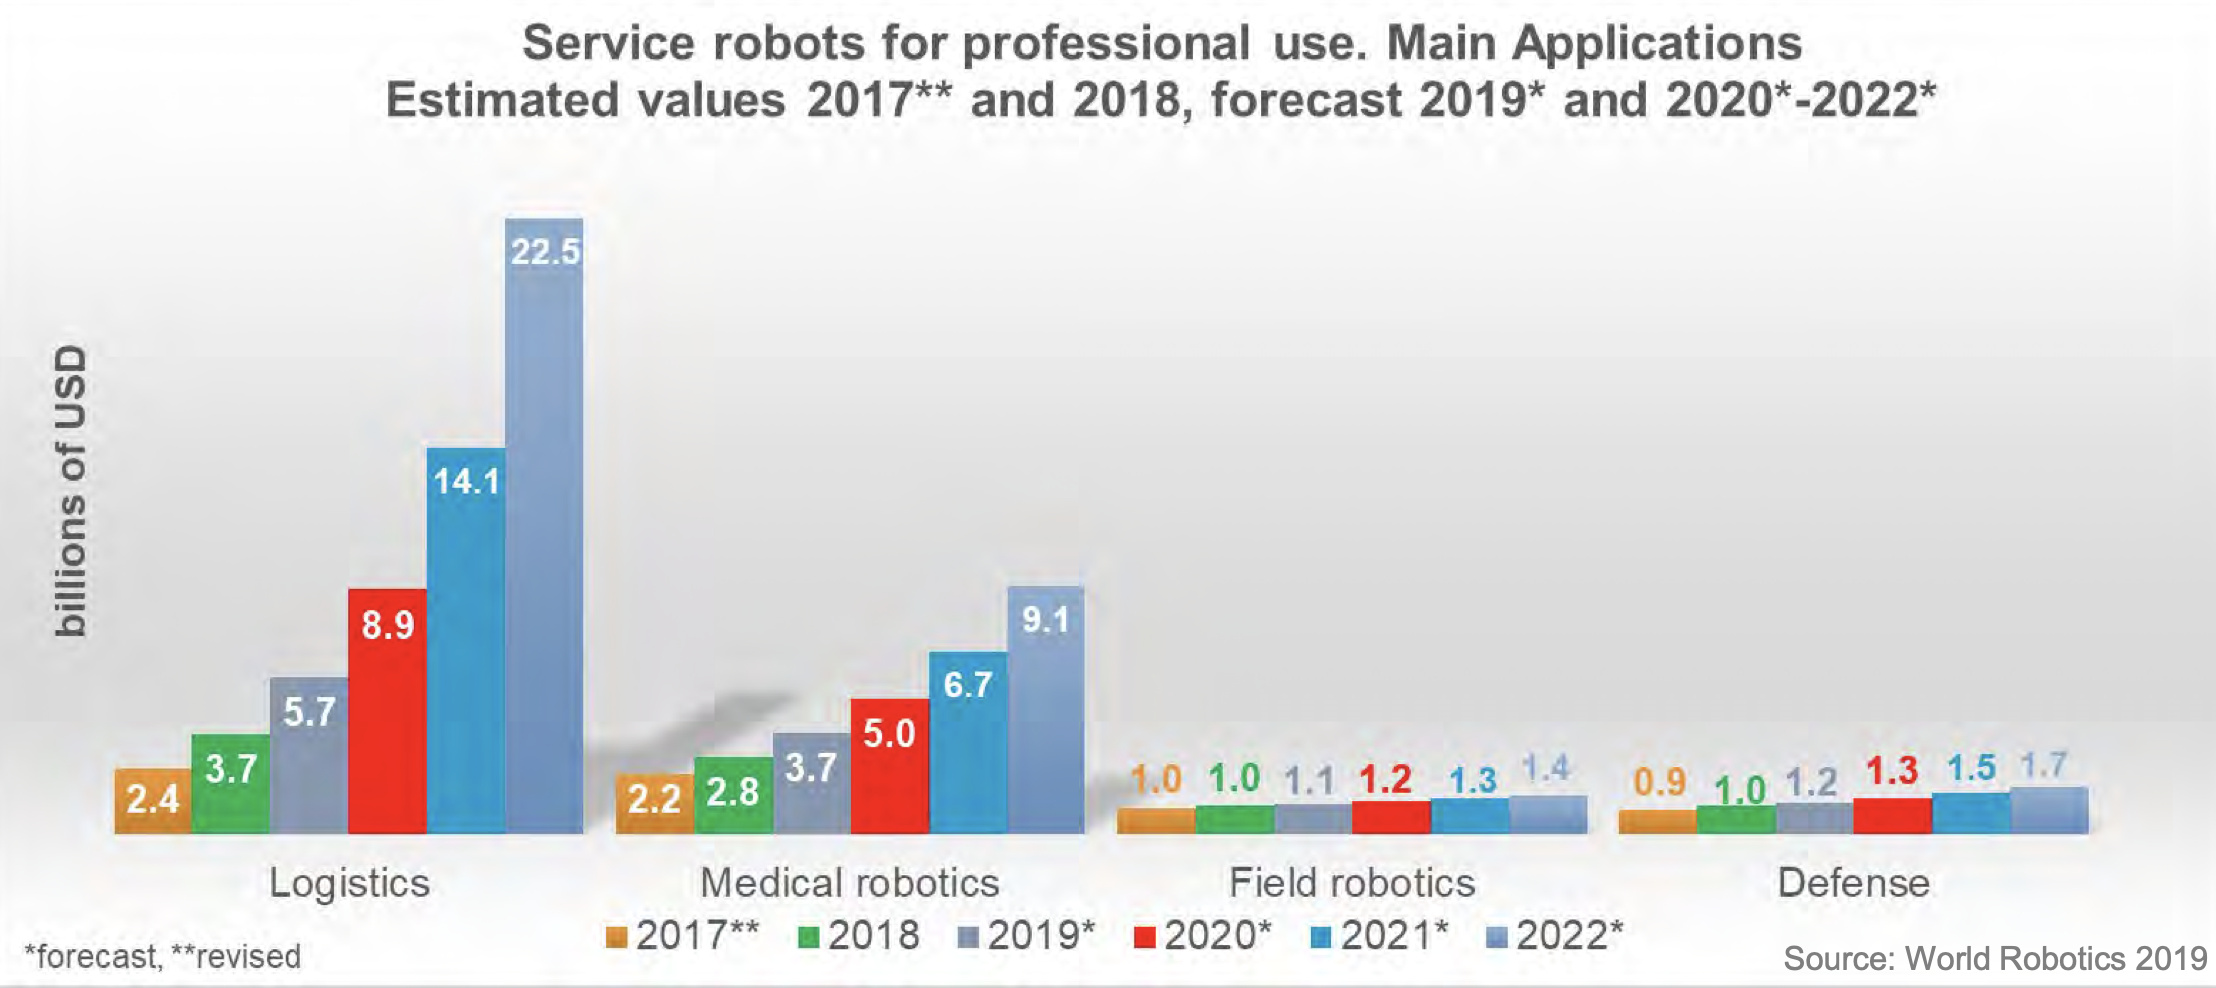
\includegraphics[width=\imgwidth]{images/service_robotics.png}
\captionof{figure}{Estimated global revenue of service robots by professional use from 2017 until 2020}
\label{img:service_robotics}
\end{center}
\end{figure}

A blog article published by the Management Review of MITs Sloan School stated that this development might be vastly accelerated due to the societal effects of COVID-19.\footnote{\href{https://sloanreview.mit.edu/article/ai-robots-and-ethics-in-the-age-of-covid-19/}{AI, Robots, and Ethics in the Age of COVID-19 - MIT Sloan Management Review}} A perfect example of this development can be observed in the Bishan-Ang Mo Kio park in Singapore, where the robot dog "Spot" is patrolling to monitor social distancing measures. While in the example the robot still is piloted by a human controller, in future these systems should work fully autonomously.\footnote{\href{http://www.straitstimes.com/singapore/meet-spot-the-safe-distancing-robot-on-trial-in-bishan-amk-park}{Meet Spot, the safe distancing robot on trial in Bishan-AMK Park - The Straits Times}}

\begin{figure}[!ht]
\begin{center}
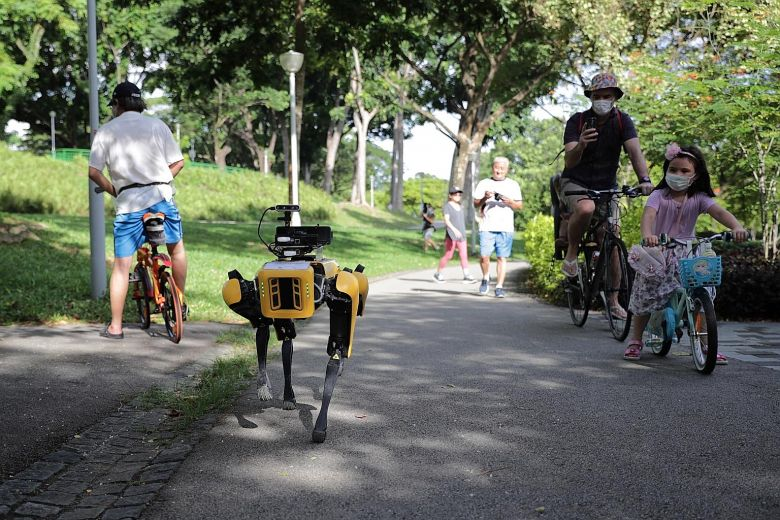
\includegraphics[width=\imgwidth]{images/spot.jpg}
\captionof{figure}{Boston Dynamics robot dog Spot patrolling in Bishan-Ang Mo Kio Park in Singapore in May 2020}
\label{img:spot_in_park}
\end{center}
\end{figure}

Summarising, robots taking part in a growing part of our social and economical life, however, an efficient but more importantly safe interaction between robots and humans is crucial for its success, interactions such as walking in between them as in the example displaying in Figure \ref{img:spot_in_park}.
\newline
In interactive multi-agent scenarios the standard control loop of percepting the sensor input, predicting, planning and executing the action \cite{Siegwart2011} is extended by a backward loop, due to the effects of the planned actions which have to be taken into account. Therefore after planning some future trajectory of the robot, a simulation predicts the behaviour of the interacting agents, conditioned on the planned robot trajectory (comp. Figure \ref{fig:control_loop_interactive}, idea from \cite{Romanski2019}). In order to guarantee interaction properties such safety usually the planner has to take into account the behaviour of the other agents. However, as the term interactive implies, this behaviour depends on the planned robot trajectory. This intrinsic dependence loop makes it especially hard to deal with interactive scenario. 

\begin{figure}
\begin{center}
\tikzstyle{block} = [draw, rectangle, minimum height=3em, minimum width=6em]
\tikzstyle{sim} = [draw, fill=cyan, rectangle, minimum height=3em, minimum width=6em]
\tikzstyle{input} = [draw, fill=orange, rectangle, minimum height=3em, minimum width=6em]
\tikzstyle{output} = [draw, fill=yellow, rectangle, minimum height=3em, minimum width=6em]
\begin{tikzpicture}[align=center, node distance=3cm,>=latex']

    \node[input, name=input](input){Sensor Input};
	\node [block, right of=input] (perception){Perception};
    \draw [->] (input) -- node {} (perception);
	\node [block, right of=perception] (prediction){Prediction};
	\draw [->] (perception) -- node[name=x] {} (prediction);
	\node [block, right of=prediction] (planning){Planning};
    \draw [->] (prediction) -- node[name=y] {} (planning);
	\node [sim, below of=y] (simulation){Simulation};
	\node [output, right of=planning] (actors){Actors};
	\draw [->] (planning) -- node[name=z] {} (actors);
	\draw [->] (z) |- (simulation);
	\draw [->] (simulation) -| (x);

\end{tikzpicture}
\captionof{figure}{Robotics control loop for interactive multi-agent scenarios}
\label{fig:control_loop_interactive}
\end{center}
\end{figure}

Within the field of safe navigation in crowded areas, especially in for human crowds. While humans use their "theory of mind", for reasoning about the other human's actions \cite{Gweon2013}, robots do not have this capacity (so far). As a consequence approaches that act in this highly dynamic, uncertain and multi-modal environment try to reduce the complexity of the problem by making strong assumptions about the human behaviour and/or by avoiding any risk. These approaches lack at least one of these properties, that are crucial for working reliable and safe near humans: 

\begin{itemize}
\item Realistic representation of the real, complex human behaviour including its multi-modal, probabilistic and highly dynamic nature
\item Certifiability by being able to explain and predict the outcome (or at least bounding it) in order to guarantee safety 
\item Computational efficient for real-time application
\end{itemize}

When walking in crowded areas humans use their theory of mind, giving them the capability to infer the actions of oncoming agents \cite{Ivanovic2018} \cite{Gweon2013}. In order to navigate through the crowd while avoiding the others as best as possible then using the inferred information the human steers into local minima regarding both the required travel time to reach some goal and avoiding the other pedestrian. In this way, as everyday life shows, the human way of walking naturally combines efficiency and safety. Although safety measures are not explicitly "optimised" collisions are prevented by reducing the amount of interaction, so that possibly un-safe scenarios are omitted before they can evolve instead of trying to contain safety within the interaction. Thus, in this project these behaviour should be imitated by minimising both the estimated travel time and a cost for minimising the interaction in parallel, while being informed by a "theory-of-mind"-like pedestrian prediction model. 


\section{Goals}
\label{text:introduction/goals}
In this work I want to tackle safe navigation in human crowds by combining two of the main paradigms in this field, trajectory optimisation algorithms and deep learning prediction models. I want to come up with an algorithm that both takes the complex human behaviour into account, without the need of strong assumptions about human behaviour, while still being able to track and guarantee properties of the resulting robot trajectory. Also I want to re-frame the problem of safe navigation from pure travel-time or safety optimally to an interaction-aware objective, minimising the disturbance the robot causes on the human behaviour, e.g. to not disrupt doctors in an hospital floor or the pedestrians strolling in the park mentioned above, while guaranteeing safety and reaching the goal when possible.
\newline
Therefore I will use a state-of-the-art deep learned probabilistic and multi-modal pedestrian trajectory prediction model combined with a shooting trajectory optimisation algorithm. To inform the gradients of its objective function, I will not use the model's output but the prediction models internal structure itself in order to optimally exploit the "hidden" information about the interactions with other pedestrians and the robot that are stored in the latent representations of the deep learned model. Thereby the main objective of the algorithm is not to reach the goal in the smallest possible robot travel-time, but to disturb the surrounding humans as less as feasible while still reaching the robot's goal. Additionally, a Hamilton-Jacobi reachability based constraint will be used for guaranteeing a safe interaction. The algorithm should be real-time feasible running with a frequency of $10 Hz$, similarly to related work discussed in chapter \ref{text:related_work} (e.g. \cite{Chen2017}).


\section{Outline of Work}
\label{text:introduction/outline}
This thesis contains five parts. Chapter \ref{text:introduction} motivates this work and provides insights into the challenges as well as possible applications, defines its goals and gives a brief overview of the solution developed within the thesis. Chapter \ref{text:related_work} introduces the reader into related work in the areas of pedestrian prediction model, controls \& decision making algorithms focussing on interaction between robots and humans, types of trajectory optimisation algorithms and to technical notions of safety. Chapter \ref{text:approach} deep dives into the algorithm developed within this work, starting with a more detailed summary and continuing with a detailed description and explanation of every of its parts. Chapter \ref{text:experiments} validates the approach by presenting experimental results for different settings and scenarios, measuring its performance on baselines and discussing the results. Finally, chapter \ref{text:conclusion} concludes the work and gives an outlook for future research directions.

\section{Statement of Contributions}
\label{text:introduction/contributions}

%todo: statement of contributions

\chapter{Related Work}
\label{text:related}
Socially-aware and safe navigation among human pedestrians poses a problem which is far from being solved and applicable to a wide range of real-world scenarios. One of the challenging factors of this field lies in the broad palette of building blocks that a possible solution may depend on, each being a challenging subproblem. In the following, some of the related subproblems tackled within project \project are introduced.

\section{Pedestrian Prediction}
\label{text:related/prediction}
The problem of predicting human motions has been tackled by many different approaches. Some approaches try to model the human dynamics, including the dynamics of their interaction with their environment, or try to come up with a cost function that the human is trying to maximize (ontological methods). Other approaches model the pedestrian behavior merely by observing and (afterward) replicating it, without the use of inherent assumptions about the structure of the interaction or the human mindset itself (phenomenological methods).

\subsection{Ontological Approaches}
As described above, ontological approaches tackle the problem of predicting human movement by describing it as guided by an underlying "physical" model or some cost function. One popular example of a "physics-based" model, i.e., algorithms that model the pedestrian dynamics using first-order physical principles, is the social forces model \cite{Helbing1995}. The Social Forces model is one of the most commonly used pedestrian predictions models in the field, due to its combined capabilities to accurately predict the behavior of human movement, its tractability, and its small computational complexity. The model uses first-order mechanical principles for forecasting the human motions in accordance with several interaction forces, that describe the impacts the pedestrian is exposed to:

\begin{align}
\vec{F} &= \underbrace{\frac{1}{\tau_{\alpha}} (v^0_{\alpha} \vec{e}_{\alpha} - \vec{v}_{\alpha})}_{F_{goal}} - \underbrace{\nabla_{\vec{r}_{\alpha \beta}} V_{\alpha \beta}[b(\vec{r}_{\alpha \beta})]}_{F_{interaction}} 
\label{eq:social_forces} \\
2b &= \sqrt{(||\vec{r}_{\alpha \beta}|| + ||\vec{r}_{\alpha \beta} - v_{\beta} \dt \vec{e}_{\beta}||)^2 - (v_{\beta} \dt)^2}
\end{align}

For every pedestrian $\alpha$, Social Forces describes an attractive force to reach an imaginary goal position with desired velocity $v^0_{\alpha} \vec{e}_{\alpha}$, with $\vec{e}_{\alpha}$ being the unit direction vector pointing from the pedestrian's current to its goal position and $v^0_{\alpha}$ being the desired speed, e.g.,\ the maximal speed. The second force describes the repulsive forces the pedestrians exert among each other, modeled by the gradient of some potential field $V_{\alpha \beta} = V_{\alpha \beta}^0 \exp(-b / \sigma)$ in the direction pointing from pedestrian $\alpha$ to pedestrian $\beta$. Thereby, $b$ takes the relative speed and directions of the regarded pedestrian pair into account. While Social Forces is a mainly deterministic model, similar approaches use recursive Bayesian filtering to deal with uncertainty, such as \cite{Schneider2013}\cite{Rehder2015}\cite{Guo2016}. Due to the small computational complexity and the high tractability of these models, they tend to be very useful for large scale simulations but are prone to modeling errors in small scale predictions, as they widely hinge on a set of estimated parameters which is assigned individually to each pedestrian, might not grasp the exact dynamical model of the pedestrian and do not take into account knowledge about past interactions, which is likely to be important for the up-coming interactions.
\newline
Another way of explicitly formulating the humans' interaction with their environment is by deriving a cost function that the human maximizes during the interaction. While some works describe the cost function as a payoff of a cooperative or adversarial game and apply game theory to predict the behavior of the other agents as well as of the agent itself, such as \cite{Bouzat2014}\cite{Nikolaidis2017}, other works use \ac{IRL} \cite{Ng2000} to characterize the interaction as a value function assigned to each state-action-pair, such as \cite{Fahad2018}\cite{Fernando2019}\cite{Saleh2018}, or as an expansion to probabilistic predictions using maximum entropy \ac{IRL} \cite{Ziebart2008}. Since IRL-based approaches rely on the Markovian property, they are not capable of including the interaction history while losing the property of tractability by using a sufficiently complex reward function for modeling human interaction. Consequently, these approaches might work well under the constraints of limited data due to the possibility of encoding prior knowledge and the extrapolation capabilities of \ac{IRL}-based approaches but lack behind phenomenological in the presence of many available data.

\subsection{Phenomenological Approaches}
Phenomenological methods incorporate data-driven techniques to observe and imitate human behavior. As a consequence, they make merely minimal assumptions about the inherent interaction process, especially in comparison to most of the ontological methods discussed above. Therefore, the availability of a reasonably large set of observable data is the key to developing a well-performing prediction model. However, since increasingly many pedestrian datasets became available over recent years, such as \cite{Pellegrini2009}\cite{Rasouli2019}\cite{Caesar2020}, phenomenological models became increasingly accurate for a wide range of scenarios. 
\newline
In contrast to previously described methods, phenomenological approaches do not assume Markovian state transitions and are therefore capable of taking the state histories of each agent into account, a presumably crucial feature for a precise prediction over future states. \ac{LSTM} modules \cite{Hochreiter1997} have been developed to model temporal sequences and are thus perfectly suitable for the purpose of mining past human trajectories for predicting future states, as done in \cite{Chen2019a}\cite{Hug2018}\cite{Zhang2019}\cite{Jain2016} (similarly using GRUs \cite{Liu2020}). However, the resulting deterministic trajectory output is not able to account for the uncertainty assigned to each prediction of future states, particularly due to the dynamic nature of human gait. To fully account for each possible future outcome, however, unimodal predictions would either miss some eventualities or be overly conservative estimates. 
\newline
Generative models proved to be well applicable to solve this dilemma by producing general (including multi-modal) probability distribution over future pedestrian trajectories, learned from data. A \ac{GAN} \cite{Goodfellow2014}, a type of (deep) generative models, has been widely used in the field, as in \cite{Gupta2018}\cite{Kosaraju2019}\cite{Ouyang2018} but is especially hard to train due to the internal conflict between generator and discriminator and generally output empirical distributions. Related to \ac{GAN}s are \ac{VAE}, a class of generative models that make use of a latent space. Conditional VAEs (CVAEs) have been recently used to predict distributions over pedestrian trajectories. CVAEs can learn the probability distribution of their latent space variables and map samples of these distribution to obtain a desired output distribution, allowing empirical as well as analytical distributions, and being easier to train in comparison to \ac{GAN}s. Especially, this only allows to formulate the desired output distribution to be processable for online usage. Examples of works using (C)\ac{VAE}s in the area of pedestrian prediction are \cite{Ivanovic2018}\cite{Salzmann2020}\cite{Poibrenski2020}\cite{Lee2017}.

\subsection{Trajectron}
The Trajectron++ model \cite{Salzmann2020} by Salzmann et alt., an enhancement of the original Trajectron model \cite{Ivanovic2018}\footnote{For the sake of brevity in the following the Trajectron++ model will be addressed by the Trajectron model.}, is a generative, graph-structured, pedestrian prediction model based on a C\ac{VAE}. By incorporating the state histories of various agents in the scene as well as their environment, it can efficiently predict a distribution over a full trajectory of future states, each being multi-modal and represented by a \ac{GMM}. Especially, to the best of the authors' knowledge, the Trajectron model is the only model within the field of pedestrian prediction that is able to condition the prediction on a robot's planned trajectory.

\begin{figure}[!ht]
\begin{center}
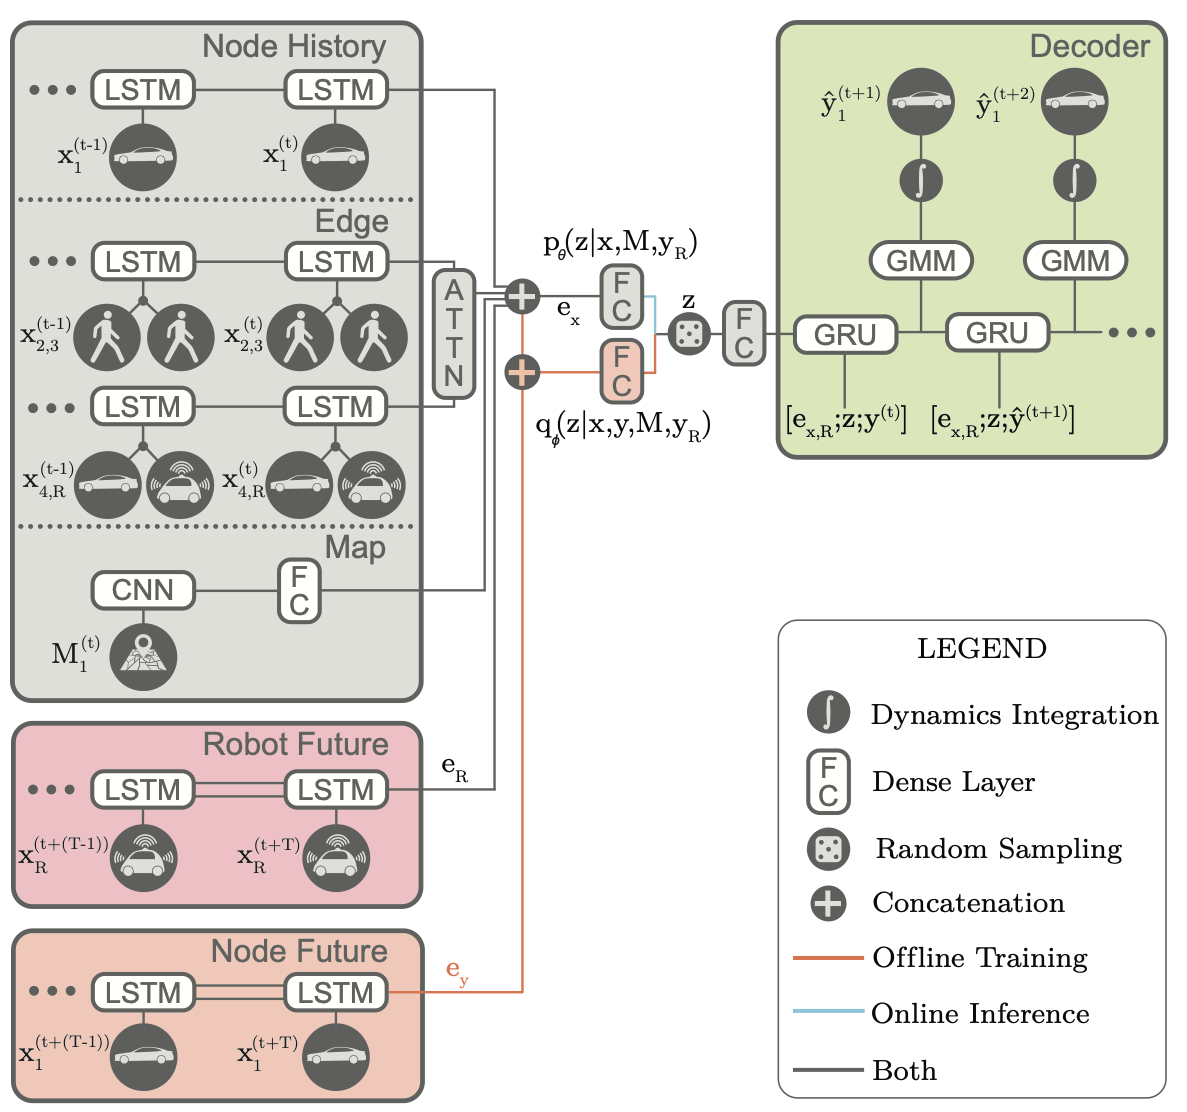
\includegraphics[width=\imgwidth]{images/trajectron++.png}
\captionof{figure}{Spatiotemporal network architecture of Trajectron++ model \cite{Salzmann2020}}
\label{img:trajectron_model}
\end{center}
\end{figure}

\begin{equation}
\max_{\phi, \theta, \psi} \sum_{i=1}^N \mathbb{E}_{z \sim q_{\phi}(z | x_i, y_i)} [\log p_\psi (y_i | x_i, z)] - \beta D_{KL} (q_{\phi}(z | x_i, y_i) || p_{\theta}(z | x_i)) + \alpha I_q(\boldsymbol{x}; z)
\label{eq:trajectron_loss}
\end{equation}

Figure \ref{img:trajectron_model} shows the architecture of the Trajectron model. Each agent in the scene is modeled as a node in a spatio-temporal graph, with assigned state history and properties shared by nodes of the same type, e.g.,\ pedestrian or vehicle. Equation \ref{eq:trajectron_loss} shows the loss function the model is being trained with. In the first step, the inputs, which are the state history of each node, including the robot, the environment obstacle map, as well as the planned robot trajectory (inputs $\boldsymbol{x}$), are encoded to a 25 dimensional latent space $\boldsymbol{z}$. The latent space representation is then sampled to generate the output distribution $\boldsymbol{y}$, unrolled over the full prediction horizon. Formally, the model is described as estimating the conditional probability distribution $p(\boldsymbol{y}|\boldsymbol{x})$ by marginalizing over the latent variable $\boldsymbol{z}$:

\begin{equation}
p(\boldsymbol{y}|\boldsymbol{x}) = \sum_{\boldsymbol{z}} p_{\psi} (\boldsymbol{y} | \boldsymbol{x}, z) p_{\theta}(z | \boldsymbol{x})
\end{equation}

The optimization can be regarded as maximizing the $\beta$-weighted evidence lower-bound of the conditional distribution $p(\boldsymbol{y}|\boldsymbol{x})$ \cite{Ivanovic2018}. Although the model is able to deal with the agent's environment as well as several types of agents project, \project focuses on the pedestrian type in a free-space environment, which is described in Section \ref{text:approach/formulation} and its implications in Section \ref{text:experiments/integration}.

\section{Safe Planning under Uncertainty}
\label{text:related/uncertainty}
Trajectory optimization itself is a wide field with many different methodologies. Though the area can be roughly broken down into two categories, shooting and collocation \cite{Kelly2017}.\footnote{There are several other directions of separation possible such as the direct vs indirect methods, but I will focus on shooting vs collocation here. Further information about the taxonomy of trajectory optimization can be found in \cite{Kelly2017}  and \cite{Chai2020}.} Shooting optimizes for the control inputs and unrolls them using a simulation environment to compute objective and constraint. Thereby, the dynamics constraint $x = \f(x, u)$ is intrinsically enforced. In comparison, collocation uses all controls and states as decision variables while constraining the system dynamics and tries to solve the \ac{NLP} by approximating some function (e.g.\ Lagrange polynomials in orthogonal collocation).
\newline
While traditionally, the problem of trajectory optimization under uncertainty has been tackled by using fixed error bounds on all uncertainties in the system, which is also known as robust control \cite{Bemporad1999}. Consequently, solutions obtained were largely sub-optimal due to widely overestimating the actual system uncertainties, or the optimization formulation became infeasible and thus impossible to solve. Subsequently, many different directions of research have evolved, such as formulating the problem as a \ac{POMDP} and (online) \ac{POMDP}-solvers to find feasible trajectories \cite{Chen2016}, using Monte-Carlo planning \cite{Janson2015} \cite{Silver2010}, signal temporal logic \cite{Sadigh2016}, (probabilistic) decision graphs \cite{Koenig1994}, sampling-based methods, as well as constraint formulations that estimate and bound the risk (or chance) of collision \cite{Ono2015}\cite{Lew2019}\cite{Chow2015a}\cite{Chow2013}\cite{Ono2012}\cite{Ludersa}\cite{Luders2011}\cite{Otte2014} or reachability-based concepts for guaranteeing the impossibility of collision solely on the base of the dynamical properties and initial conditions of interacting agents \cite{Leung2020}\cite{Dhinakaran2017}\cite{Margellos2009}\cite{Chen2017b} \cite{Althoff2009}\cite{Althoff2010}. Since discussing all of these different techniques surely is out of the scope of this work, only three approaches, which are most relevant to this work, will be examined in the following:

\subsection{Sampling-based Path Planning}
Sampling-based path planning methods, such as RRT \cite{LaValle1998}, have been shown to be an efficient solution for path planning in continuous-space, static environments, while often guaranteeing asymptotic optimality and feasibility of the derived solution, such as \cite{Karaman2011}\cite{Luders}. These algorithms are iteratively sampling random points from the configuration space, while retaining those in the free space (i.e., free from obstacles), storing them as milestones in a roadmap, and connecting those milestones, which can be connected completely in the free space. The algorithm repeats until either the goal state has been incorporated in the roadmap or the maximal computation time has exceeded. To account for dynamic and probabilistic obstacles, a temporal dimension has to be added to the search space, making the problem computationally challenging to solve in real-time. For addressing this issue, rapid replanning and repairing \cite{Otte2014} are often used. To implicitly take into account system uncertainties, the occupancy cost can be augmented by risk level sets that assign a certain risk to each robot state, depending on the obstacle's state, e.g., its orientation and velocity, as shown in \cite{Pierson2018}\cite{Pierson2019}. However, despite the success of sampling-based methods in online path planning, they do not explicitly leverage future predictions of the environment and are therefore restricted to only (temporally) locally optimal solutions.

\subsection{Chance Constraints}
Chance constraints are a specific way of formulating a constraint under uncertainty, such that it holds for at least a pre-defined probability level $p$. With a general inequality constraint $g(x) \leq 0$ it is:

\begin{equation}
Pr(g(x) \leq 0) \geq p
\label{eq:chance_constraint}
\end{equation}

Usually, constraint \ref{eq:chance_constraint} is reformulated as a set of deterministic constraints to be manageable for optimization. Therefore, several methods have been purposed: Sampling-based methods relying on the Bernstein approximation \cite{Calafiore2005}, on scenario planning approach \cite{Bemporad1999}, or Monte Carlo sampling \cite{Hong2011}\cite{Janson2015} as well as dynamic-programming based approaches for discrete space \cite{Chow2013}\cite{Ono2015} \cite{Chow2015a}. While these methods work for general distributions but are usually too slow for an online optimization approach, shrinking the space of distributions can improve the performance, such as in \cite{Chen2018}\cite{Calafiore2006}\cite{Carvalho2014}\cite{Blackmore2009}\cite{Blackmore2011}. Thereby, handling multi-modality of the risk distribution efficiently is a widely untouched ground, to the best of the authors' knowledge, which only has been solved for a specific scenario, such as in \cite{Hu2018}. To conclude, solving a chance constraints program efficiently is quite hard to do, especially when dealing with general, such as multi-modal and non-convex risk distributions.

\subsection{Hamilton-Jacobi Reachability} 
Reachability analysis deals with the problem of a two-person, zero-sum differential game. Specifically, it tries to solve the question how to react if there is another player that interferes with the fulfillment of the robot's objective by optimizing the joint system state, assuming that the counter-player always counters the robot's action optimally, i.e., assuming the worst case disturbance $\d = \beta[\u]$ \cite{Pavone2020}. Under these conditions, the optimal control strategy can be derived by maximizing: \\

\begin{equation}
V(x(t), t) = \min_{\beta[\u](\cdot)} \max_{\u(\cdot)} \left[ \int_t^0 l(\x(\tau), \u(\tau), \boldsymbol{d}(\tau)) \, d\tau + l_f(\x(0)) \right]
\label{eq:j_reachability}
\end{equation}

with $(\x(\tau), \u(\tau), \d(\tau))$ describing the joint system with dynamics $f(\boldsymbol{x}, \u, \d)$. While solving the robot's optimal control strategy $\u_{opt}$ in open-loop (also \textit{forward} reachability) is computationally inexpensive but leads to overly conservative and hence un-realistic estimates, since the counter-player knows the entire policy $\u_{opt}$ in advance and can re-act accordingly, \ac{HJR} (also \textit{backward} reachability) addresses the problem of maximizing Equation \ref{eq:j_reachability} in closed-loop, i.e., by allowing the robot to adapt its control policy at each time-step. As proven in \cite{Pavone2020}, this is equivalent to solving the Hamilton-Jacobi-Isaacs differential equation with boundary condition: \\

\begin{problem}{General \ac{HJR} problem}
\begin{align}
\pd{V}{t} + \max_{\u}  \min_{\d} &\left[l(\x, \u, \d) + \nabla V^T f(\x, \u, \d) \right] = 0 \\ 
V(\x, 0) &= l_f(\x) \\
\Rightarrow \u_{opt} &= \arg \max_{\u}  \min_{\d} \nabla V^T f(\x, \u, \d)
\label{eq:hjr_problem_u}
\end{align}
\label{eq:hjr_problem}
\end{problem}

Solving Problem \ref{eq:hjr_problem} has been examined for several scenarios and applications over the recent years, as in \cite{Dhinakaran2017}\cite{Margellos2009}\cite{Chen2017b}, and has shown to be especially useful in the field of autonomous driving \cite{Althoff2009}\cite{Althoff2014}\cite{Althoff2010}. In opposite to forward reachability, \ac{HJR} finds the non-overly conservative avoidance maneuvers, "stemming from its equivalence to an exhaustive search over the joint system dynamics" while still being flexible with respect to the system dynamics, as depicted by \cite{Leung2020}. To solve \ref{eq:hjr_problem}, the value function $V(\cdot)$ as well as its gradient are computed for every cell of a $n$-dimensional grid that discretizes the joint state $\x(\tau)$ and for some discrete time horizon (including $\tau \rightarrow \infty$). 

\section{Navigation in Human Crowds}
\label{text:related/crowd_navigation}
Navigation in human crowds is especially important for vastly integrating autonomous ground vehicles in our daily life but poses a hard problem due to a priori unknown human intentions and hard to quantify objectives, e.g.,\ the notion of socially-acceptable behavior. Existing work in this field can be roughly divided into two main directions, model- and learning-based approaches: 

\subsection{Model-Based Approaches}
Traditionally, the pedestrians are regarded as dynamic obstacles, with the collision avoidance algorithm being used for robot navigation \cite{vandenBerg2011}\cite{Fox1997}\cite{Luo2018a}\cite{Phillips2011}. \ac{ORCA} \cite{vandenBerg2011}, for example, guarantees a collision-free pre-defined time horizon, under the assumption of perfect knowledge about the state of each interacting agents as well as, more importantly, a shared, deterministic policy over all agents. Although these models have been advanced to relax some of the assumptions such as perfect perception \cite{Hennes2012}, they still fail to capture a human-like behavior and, consequently, may lead to unsafe and socially unacceptable robot actions. To solve this issue, it is crucial to directly include the predicted impact of the robot's planned trajectories into the optimization itself. For this reason, the robot's motion has been incorporated in some of the (model-based) pedestrian prediction models discussed in Section \ref{text:related/prediction}, e.g.,\ the Social Forces model \cite{Helbing1995}, usually by augmenting the model by robot-specific parameters while preserving the general concept of interaction \cite{Ferrer2013}\cite{Luo2018a}. Nonetheless, as discussed, these models usually are largely hinging on parameters, making them hard to tune and hence inaccurate in prediction and thus planning as a consequence of modeling errors. Additionally, model-based approaches are usually deterministic, regarding only one out of assumably many possible outcomes, and therefore might lead to un-safe behavior.

\subsection{Learning-based Approaches}
Learning-based approaches try to replicate human behavior that has been learned from human demonstration in simulations or by accumulating features over possible trajectories of interacting agents while minimizing some interactive cost function (e.g.,\ the separation distance) \cite{Kim2016}\cite{Kretzschmar2016}. While these models tend to plan trajectories that are more socially acceptable and natural, they are much larger in computational cost and very hard to train due to the dynamic and stochastic nature of human gait. Other approaches come up with a set of socially compliant rules, such as "passing on the right" and use deep reinforcement learning to apply them  \cite{Knepper2012}\cite{Chen2017}\cite{Everett2018}. However, it can be doubted whether these methods can be generalized to unseen scenarios, how to certify a safe interaction, and whether these rules hold at all.
\newline\newline
While model-based approaches are computationally efficient and tractable but lack an accurate capturing of human behavior, learning-based methods do model the human motion more naturally and are therefore capable of planning socially-aware trajectories. However, they tend to be computationally expensive, are neither tractable nor able to give any safety guarantees, which is crucial for secure human-robot interaction. Therefore, this works wants to combine both worlds, the predictive abilities of deep learned models with the safety guarantees of model-based safety guaranteeing methods, such as \ac{HJR}, which was discussed above. To truly leverage the full "knowledge" of the prediction model, concepts of model-gradient informed concepts, which have been already shown to be successful in control theory \cite{Chen2019}\cite{Fan2020}, are thereby re-formulated for trajectory optimization. While most of the described approaches deal with deterministic and uni-modal predictions, due to the highly stochastic human motion, anticipatory and efficient, but safe interactions can only be derived when the system can reason about many possible future outcomes of the scenario so that multi-modality should be taken into account.

% sequential-action control \cite{Nishimura2020}\cite{Nishimura2020a}
\chapter{Multi-Modal Interaction-Aware Trajectory Optimization}
\label{text:approach}
In this chapter, an overview of the approach is provided. Starting in Section \ref{text:approach/formulation} the problem of socially aware motion planning is formulated formally, including the assumptions made within this project. 
\newline
Section \ref{text:approach/overview} which presents an overview of the full trajectory optimization pipeline. It is shown how the algorithm is built to allow to deal with general graph-like pedestrian behavior prediction models, with multi-modal, probabilistic outputs. Furthermore, the advantages of formulating socially aware motion planning as an optimization problem while utilizing a graph-based prediction model, e.g. deep learning-based models such as the Trajectron \cite{Ivanovic18}, over purely learned \cite{Chen2017} or purely optimization-based \cite{Berg2011} algorithms are illustrated. Finally, it is explained how the usage of a general-purpose, computation-graph based framework such as PyTorch \cite{pytorch} or TensorFlow \cite{tensorflow} can be harnessed for a highly modular, efficient, and versatile implementation.
\newline
The exact formulation of the optimization problem is further explained in Section \ref{text:approach/objective} and \ref{text:approach/constraint}. Beginning with the objective function both the goal-driven and the interaction-driven parts are illustrated, together with a derivation of their gradients. Furthermore, several designs of the specific objective function are discussed. The subsequent section addresses the design of the constraints used. Likewise, several constraint function designs are compared. 
\newline
To use the system in real-world applications it must comply with several requirements. While some of these have been tackled by the optimization design, e.g. feasibility of the control limitations of the robot or safety regarding robot-human interaction, the system underlies runtime limits. To achieve this goal several runtime improvements have been implemented, which are described in Section \ref{text:approach/runtime}.


\section{Problem Formulation}
\label{text:approach/formulation}
In this work, we are interested in finding the optimal trajectory for a robot navigating among pedestrians on the two-dimensional plane. Let $\x_t = (x_t, y_t) \in \mathbb{R}^2$ and $\dx_t = (\dot{x}_t, \dot{y}_t) \in \mathbb{R}^2 $ be the position and velocity of the robot, also referred to as $ego$, at time $t$ and $(\x, \dx)_{0:N}$, a trajectory over multiple position-velocity-pairs $((\x, \dx)_0, (\x, \dx)_1, (\x, \dx)_2, \hdots, (\x, \dx)_N)$. Within this work, the robot is assumed to have double integrator dynamics. With control input $\u_t = (u_{x, t}, u_{y, t}) \in \mathbb{R}^2$, we have: 

\begin{equation}
\ddx_t = \u_t
\label{eq:robot_dynamics}
\end{equation}

For further simplification, the robot's dynamics are assumed to be deterministic. 
The pedestrians (also referred to as $ados$) follow single integrator dynamics. As pointed out in \cite{Ivanovic2018}, this is a natural choice "as a person's movements are all position-changing, e.g., walking increases position along a direction, running does so faster." Other standard models for pedestrian dynamics such as Social Forces \cite{Helbing1995}, however, regard the pedestrian to be a double integrator, not a single integrator, and describe the forces acting on it introduced by other pedestrians and obstacles. Having a reasonable fast reaction time and a large maximal acceleration in comparison to the robot, both of these descriptions converge so that the single integrator model is the right choice nonetheless. \footnote{As discussed in Chapter \ref{text:experiments} the modular implementation allows us to use different pedestrian dynamics. When testing against other prediction environments non-single integrator dynamics are used, but most analysis described in this report relates to the single integrator model.}

\begin{align}
\dxped[k]_t = \uped[k]_t
\label{eq:pedestrian_dynamics}
\end{align}

Each pedestrian's future trajectory is predicted as a probabilistic and multimodal using some model $\distmodel[]$. Thereby, let $\xped[k]_t \sim \dist[k]_t$ be the distribution of the pedestrian $k$s velocity at time $t$, with mean $\muped[k]_t$, variance $\sigmaped[k]_t$, and mode-weights vector $\piped[k]_t$. The prediction is based on the past states of the robot $\x_{0:t}$ and of every pedestrian in the scene $\xped[j]_{0:t}$, including pedestrian $k$. Moreover, the function $\distmodel[]$ is generally not shared across all pedestrians but individually for each one.

\begin{align}
\xped[k]_t &\sim \distmodel[k]_t(\muped[k]_t, \sigmaped[k]_t, \piped[k]_t) \\
\dist[k]_t &= \distmodel[k] (\x_{0:t}, \xped[0]_{0:t}, \hdots, \xped[K]_{0:t})
\end{align}

Like the robot, the pedestrians are modeled as single point masses, both underlying speed bounds defined by the $L_2$ norm of their velocities. Furthermore, both the robot and the pedestrians underly constraints for their minimal and maximal control effort. Thus, the sets of feasible control inputs $
\uset$ and $\upedset$ respectively, are defined using the $L_1$-norm and the $L_2$-norm respectively:

\begin{align}
\uset &= \{\u | \u \in \mathbb{R}^2, ||\u||_1 \leq u_{max}\} \\
\upedset &= \{\uped[] | \uped[] \in \mathbb{R}^2, ||\uped[]||_2 \leq \tilde{u}_{max}\} 
\label{eq:controls_bounds}
\end{align}
 
All actions are assumed to take place in a free-space, two-dimensional environment. 
\newline
Within project \project, we want to find a robot trajectory $\x_{0:T}$ over some discrete-time horizon $N$ that makes trade-offs between minimizing the travel time from its current state to some goal state in $\xset_f = \{\boldsymbol{g} | \boldsymbol{g} \in \xset \}$ on the one side and the interference with the pedestrians in the scene, concerning its dynamic as well as safety boundaries, on the other side. For further simplification, perfect knowledge about the current and all past states of surrounding agents $\xped[k]_{0:t} \forall k \in [0, K]$ is assumed.
\newline\newline
For brevity of notation, in the following, the temporal index $t$ and the pedestrian index $k$ will be omitted when not necessary.


\section{System Overview}
\label{text:approach/overview}
As shown in Figure \ref{img:information_flow} the problem can be divided into several subproblems, which also can be seen as modules of a trajectory optimization problem and therefore can be formulated independently from each other. 

\begin{figure}[!ht]
\begin{center}

\includegraphics[width=\imgwidth]{images/placeholder.png}
\caption{Information-Flow-Diagram}
\label{img:information_flow}
\end{center}
\end{figure}

Formally, the solution to this problem can be represented as the following optimization problem (compare Problem \ref{eq:formulation}), which is executed in an MPC-manner. \\

\begin{problem}{\textrm{General optimization problem}}
\begin{equation}
\min_{\u_{0:T-1}} \quad w_{goal} J_{goal} + w_{int} \sum_{k=0}^K J_{int}^k
\end{equation}
\begin{align}
\textrm{s.t. } \quad & \x_{t+1} = \f(\x_t, \u_t) & \forall t \in [0, T - 1] \\
& \xped[k] = \distmodel[k](\x_{0:t}, \xped[i]_{0:t}) & \forall k \in [0, K], \forall t \in [0, T]\\
& g_{safety}(\x_{0:T}, \xped[k]_{0:T}) \leq 0 & \forall k \in [0, K] \\
& \x_t \in \xset & \forall t \in [0, T]\\
& \u_t \in \uset & \forall t \in [0, T]\\
& \x_0 \in \xset_0
\end{align} 
\label{eq:formulation}
\end{problem}

. Due to the linear and cheap to compute dynamics, the availability of a simulation engine tightly bound to the optimization and since the constraints acting on both the path $\x_{0:T}$ itself and the controls $\u_{0:T}$ are comparably "simple", as illustrated in Section \ref{text:approach/constraint}, shooting is used within this project. Therefore the trajectory is split up into several segments, one for each discrete discretization time step, which makes solving problem \ref{eq:formulation} easier to be solved and more robust (multiple shooting) \cite{Betts1998}. In this work the initial time $t_0 = 0$ and the final time $t_f = T \cdot \Delta t$ is used for simple notation, although not required in general \cite{Wachter2006}. 
\newline
The objective function is a weighted sum of a goad-driven $J_{goal}(\cdot)$ and some interaction-driven term $J_{int}(\cdot)$, which are further explained in Section \ref{text:approach/objective}. The constraints are a combination of dynamics constraints, safety constraints as well as initial and final state restrictions, which are discussed in Section \ref{text:approach/constraint}. Note that the terminal state $\x_T$ of the planned trajectory is not constrained to be in the terminal set $\xset_f$. As stated in chapter \ref{text:introduction} within this project the safety and un-disturbed gait of pedestrians is considered to be more important than reaching the goal state time-optimally. While the goal-driven objective $J_{goal}(\cdot)$ introduces an incentive to approach the goal state, constraining the terminal state to be in the terminal set would informally speaking, remove the possibility of detouring to not interfere a pedestrians movement. 
\newline
Over Problem \ref{eq:formulation} has $2*T$ optimization variables, $(2*T + 1) + 2*T + K = 3*T + K + 1$ constraints, all of them being inequality constraints, causing $T * (T+1) + 2*T + K$ non-zero Jacobian elements.

\subsubsection{Nonlinear optimization Solver} 
Since no further assumptions about the pedestrian trajectory prediction model $\distmodel[]$ have been made, the optimization is non-linear and especially non-convex in general. As shown in \cite{Gould2003}\cite{Parkinson2018}\cite{Freund2004} there are a bunch of algorithms to deal with general non-linear optimization problems, such as line-search, trust-region, interior-point, generalized-reduced-gradient or sequential-quadratic-programming methods as well as combinations of these such as LOQO. However, not all of them apply to constrained problems such as Problem \ref{eq:formulation}. For constrained optimization problems \ac{SQP} and \ac{IPM} are the most popular ones, both having their advantages and drawbacks. While \ac{SQP} usually require fewer solver iterations and thus fewer function calls, they scale poorly with the number of constraints and do not guarantee that intermediate results are feasible \cite{Dehdari2013}\cite{Parkinson2018}. Although this can be an advantage in the case of computationally expensive constraints, it also leads to an infeasible solution when the algorithm is stopped for convergence. Additionally, compared to \ac{IPM} the computational time required by the solver itself is usually larger (e.g. as demonstrated in \cite{Dehdari2013}).
\newline
In project \project safety is induced by constraint, thus obtaining a feasible solution is crucial, also if the algorithm might be aborted before convergence due to runtime constraints. For this reason, an interior-point method has been used within the project. The idea of interior point optimization methods is to create constraint barriers that increasingly push the solution from an infeasible state to the feasible region, without pushing it too much away from the feasible border (since often the optimal solution is close to the feasible border), using a loss function combining the objective and constraint “loss” by introducing Lagrangian parameters. IPOPT especially has very good performance in recovering from some infeasible state in a “smart” manner.  Therefore it is quite robust, but hard to warm-start. 
\newline
The interior-point method \ac{IPOPT}\footnote{\ac{IPOPT} is only available for C++, the cython-based wrapper cyipopt is used.} \cite{Wachter2006} has shown to be applicable in many robotics applications, and has shown to be valuable even in case of very tough runtime constraints such as solving the feedforward commands in high-performance automated driving at 50 Hz in \cite{Spielberge2019} or motion planning for legged robotics \cite{Winkler2018}. Therefore it has been used in this project as well\footnote{From today's point of view it turned out, after tweaking the performance of the optimization core as best as possible, it turns out that the number of objective function calls is the bottleneck of the algorithm. Therefore comparing the capacity of the interior-point solver such as \ac{IPOPT} with \ac{SQP} solvers such as \ac{GuSTO} remains for future work.}.

% The NLP solver implements the following primal-dual methods for finding a local minimum: 1) interior point trust-region line-search algorithm 2)active-set trust-region line-search algorithm
%Both methods can solve small-, medium-, and large-scale optimization problems efficiently and robustly. These methods use exact first and second derivatives to calculate search directions. The memory requirements of both algorithms are reduced dramatically because only nonzero elements of matrices are stored. Convergence of both algorithms is achieved by using a trust-region line-search framework that guides the iterations towards the optimal solution. If a trust-region subproblem fails to provide a suitable step of improvement, a line-search is then used to fine tune the trust-region radius and ensure sufficient decrease in objective function and constraint violations.
%The interior point technique implements a primal-dual interior point algorithm in which barrier functions are used to ensure that the algorithm remains feasible with respect to the bound constraints. Interior point methods are extremely useful when the optimization problem contains many inequality constraints and you suspect that most of these constraints will be satisfied as strict inequalities at the optimal solution.
%https://documentation.sas.com/?docsetId=ormpug&docsetTarget=ormpug_nlpsolver_overview.htm&docsetVersion=14.3

\subsubsection{Implementation Details} 
The algorithm has been implemented in Python 3.7 using PyTorch \cite{pytorch}. Next to executing computations highly efficiently by vectorization and batching PyTorch's automatic differentiation framework allows computing gradients at low computational cost as well as modular, i.e.\ without the need to explicitly define its closed form. This is the core of prediction-based optimization, enabling to define objectives and constraints (such as $J_{int}$), which depend on a complex graph-based computation, and still being able to derive their gradient without costly and inaccurate numerical approximations. 
\newline 
Furthermore, the algorithm has been implemented highly modular, allowing to easily use pre-defined simulation environments, objective, constraint functions, or new solvers and switch between them without much knowledge about the underlying implementation. To pave the way for further projects based on this project it has been widely documented using Sphinx\footnote{Automated code documentation: https://www.sphinx-doc.org/en/master/}, for further information please visit the \href{https://simon-schaefer.github.io/mantrap/}{project's website}.  
\newline
The system's integrity has been verified by roughly 500 unit- and integration tests, secured over the code developed by the continuous integration framework CircleCI\footnote{Automated testing framework: https://circleci.com} and CodeCov\footnote{Testing coverage reports: https://codecov.io}.


\section{Objective Function Design}
\label{text:approach/objective}
\subsection{Goal Objective}
\label{text:approach/objective/goal}
The goal objective gives an incentive for the optimizer to choose a solution that targets the goal state. It simply consists of the squared L2-norm between each robot trajectory point and the goal state $\goal$, normalized over the full planning horizon $N$:

\begin{equation}
J_{goal}(\x_{0:T}) = \frac{1}{T} \sum_{t = 0}^T (\x_t - \goal)^2
\label{eq:goal_unweighted}
\end{equation}

By normalization, the cost is independent of the length of the planning horizon $T$ and thus allows us to use the same weight $w_{goal}$ for different planning horizons.

\subsubsection{Horizon weighting}
Intuitively, as discussed in Chapter \ref{text:introduction} for socially aware navigation socially-aware objectives should be higher weighted than traditional control effort or travel time objectives. This is especially true at the beginning of the planning horizon. For this reason the a horizon dependent weighting $\lambda_t$ is introduced into the stage cost of the goal objective, which is small at the beginning of the horizon and large at its end: 

\begin{equation}
J_{goal}(\x_{0:T}) = \frac{1}{T} \sum_{t = 0}^T \lambda_t (\x_t - \goal)^2
\label{eq:goal_weighted}
\end{equation}

As shown later on this modification empowers a fast convergence to evasive movements of the robot, when necessary to avoid un-safe situations, while properties of $J_{goal}(\cdot)$ such as most importantly convexity remain unchanged. In Table \ref{table:goal_horizon_weighting} the convergence speed of both the "un-weighted" and the "weighted" objective formulation are compared over 100 runs in a simplified setup, with no pedestrian in the scene and random assignments of the robot's initial and goat state. Weighting the cost terms non-uniformly over the horizon enables finding "trade-offs" of a locally higher cost for a faster global convergence such as gaining speed in a non-goal-direction at the beginning of the horizon but leads to a smaller cost at the end of it. 

\begin{table}[!ht]
\begin{center}
\begin{tabular}{c|c|c}
 & Weighted & Un-Weighted \\
\hline
Avg. number of solving iterations & 9.58 & 9.64 \\
\hline
Avg. $95 \%$ decay of objective value & 5.86 & 6.64 \\
\end{tabular}
\caption{Comparison of key performance parameter of the optimization using either the "un-weighted" (Equation \ref{eq:goal_unweighted}) or the "weighted" (Equation  \ref{eq:goal_weighted}) goal objective formulation over 100 runs in a simplified environment setup. For further details please have a look into the example notebook: \href{https://github.com/simon-schaefer/mantrap/blob/master/examples/module_goal.ipynb}{examples/module\_goal}.}
\label{table:goal_horizon_weighting}
\end{center}
\end{table}

\subsubsection{Gradient}
Since the goal objective $J_{goal}(\x_{0:T})$ is only a function of the robot's planned trajectory and the goal state, its jacobian can be derived without further knowledge of the pedestrian prediction model, merely using the (known) robot dynamics. As described in Section \ref{text:approach/overview} the robot controls are optimized. Hence by applying the chain rule we get: 

\begin{equation}
\nabla J_{goal} = \pd{J_{goal}}{\u_{0:T-1}} = \pd{J_{goal}}{\x_{0:T}} \cdot \pd{\x_{0:T}}{\u_{0:T-1}}
\end{equation}

As demonstrated, the goal-objectives gradient can be derived by multiplying the objectives gradient with respect to the robot's trajectory with the gradient of the robot's trajectory with respect to its control inputs. Since the goal-objective directly depends on the trajectory, deriving the first term is straight-forward to derive. The second term $\delta \x_{0:T} / \delta \u_{0:T-1}$ is not trivial in general, because of the iterative structure of rolling out state trajectories based on dynamics and as the robot's dynamics $\f(\cdot)$ can be arbitrary, however as described in Section \ref{text:approach/formulation} double integrator dynamics are assumed for the robot, so that the whole trajectory $\x_{0:T}$ can be expressed as function of the initial state $\x_0$ and the control inputs $\u_{0:T-1}$ only, as shown in equation \ref{eq:dynamics_stacked}. Then the term $\delta \x_{0:T} / \delta \u_{0:T-1}$ simplifies to a constant term:

\begin{align}
\pd{J_{goal}}{\x_{0:T}} &= \pd{}{\x_{0:T}} \frac{1}{N} \sum_{t = 0}^N (\x_t - \goal)^2 \\
&= \frac{2}{T} \begin{bmatrix} (\x_1 - \goal) & \hdots & (\x_T - \goal) \end{bmatrix}^T
\end{align}
\begin{align}
\pd{\x_{0:T}}{\u_{0:T-1}} &= \pd{}{\u_{0:T-1}} \begin{bmatrix} A \x_0 \\ A_n \x_0 + B_n \u_{0:T-1} \end{bmatrix} \\
&= \begin{bmatrix} \boldsymbol{0}_{n \times m} \\ B_n \end{bmatrix}
\label{eq:goal_gradient_dynamics}
\end{align}

with $A_n, B_n$ the stacked state-space description matrices as described in Section \ref{text:approach/runtime/unrolling}. 
\newline
Overall the goal objective and its gradient are very efficient, cheap to compute, having linear complexity with the length of the planning horizon $T$, and being independent of the number of pedestrians. Furthermore, it is strictly convex, which improves the optimization convergence speed. Therefore it is quite valuable for warm-starting the optimization algorithm, as further explained in Section \ref{text:approach/runtime/warm_starting}.

\subsection{Interaction Objective}
\label{text:approach/objective/interactive}
The interaction between robot and pedestrian itself is an abstract quantity and can thus hardly be used for optimization itself. To approach this problem in the following we consider a scene with the robot facing only one pedestrian, to then generalize the developed concept to interactions with multiple pedestrians.  
\newline
While it is hard to find a measure for the interaction between the robot and the pedestrian in the scene when regarding the problem in general, it can be simplified when a) focussing on one of the interacting agents and b) define the measure to vanish its value. Under these conditions, the problem can be re-formulated as decreasing the disturbance the robot induces on the pedestrian, which is a lot simpler to quantify than the abstract concept of interaction. To do so the un-conditioned\footnote{For the sake of brevity the term "un-conditioned" means not depend on the robot's state. However, the pedestrian's trajectory prediction is of course still conditioned on its state history as well as the states and state history of the other pedestrians in the scene, as described in Section \ref{text:approach/formulation}.} pedestrian's trajectory distribution $\distwo[]$ is computed, i.e. the distribution that would occur if no robot would be in the scene, and then compared to its actual conditioned trajectory distribution $\dist[]$.\footnote{When the prediction model requires the input of a robot trajectory, e.g. as an "input format" requirement of a neural network-based model, predicting the un-conditioned trajectory distribution might not be straight-forward. Using a re-trained un-conditioned model is not an option since factors causing a different distribution independent from the robot's trajectory might come into play. Thus, within the project a "pseudo"-robot is used which is located very far away from any pedestrian, hence minimizing its effect on the pedestrian's behavior.} With some general distance measure $\Delta(\cdot, \cdot)$ the interactive objective function given the robot's trajectory $\x_{0:T}$ is defined as:

\begin{equation}
J_{int}^k(\x_{0:T}) = \sum_{t=0}^T \Delta(\dist[k]_t, \distwo[k]_t)
\label{eq:objective_interaction}
\end{equation}

\begin{figure}[!ht]
\begin{center}
\begin{tikzpicture}

    \node[inner sep=0pt] (pedwo) at (-3,1)
    {
\includegraphics[width=.05\textwidth]{images/walking.png}};    
    \draw [dotted, ultra thick, name path=A] (pedwo) to[out=180, in=0] node[above] {$\xpedwo[k]$} (-8, 1);
    
    \node[inner sep=0pt] (pedw) at (-3,-1)
    {
\includegraphics[width=.05\textwidth]{images/walking.png}};
    \node[inner sep=0pt] (robot) at (-7,-1)
    {
\includegraphics[width=.05\textwidth]{images/robot.png}};
    \draw [ultra thick, name path=B] (pedw) to[out=180, in=10] node[below, sloped] {$\xped[k]$}(-8,-3);
    
    \draw[thick, decorate, decoration={brace, amplitude=20pt}] (-1.5,2) -- (-1.5,-2);

    \node[inner sep=0pt] (ped) at (5,0.5)
    {
\includegraphics[width=.05\textwidth]{images/walking.png}};
    
    \draw [dotted, ultra thick, name path=A] (ped) to[out=180, in=0] node[above] {$\xpedwo[k]$} (0, 0.5);
    \draw [ultra thick, name path=B] (ped) to[out=180, in=10] node[below, sloped] {$\xped[k]$}(0,-1.5);
        
    \tikzfillbetween[of=A and B]{blue, opacity=0.2};
    \node[] (D) at (1, -0.3){$D_{int}$};
    
\end{tikzpicture}
\end{center}
\caption{Interactive measure in case of deterministic and uni-modal pedestrian trajectory predictions, which trivially is the area enclosed by the un-conditioned (upper) and the conditioned (middle) trajectory.}
\label{img:ado_w_wo_distance_trajectory}
\end{figure}

If the pedestrian's trajectory prediction would be deterministic and uni-modal this measure simply breaks down to the distance between both trajectories which is the area enclosed by both trajectories in continuous time, as shown in Figure \ref{img:ado_w_wo_distance_trajectory}, or a sum of distance per time-step in discrete time. For probabilistic and multi-modal predictions computing the distance between both distributions is more difficult, especially when demands such as computational cost and differentiability (to be used in an optimization) have to be factored in. 

\begin{figure}[!ht]
\begin{center}
\begin{tikzpicture}

    \node[inner sep=0pt] (ped) at (5,0)
    {
\includegraphics[width=.05\textwidth]{images/walking.png}};
    \node[inner sep=0pt] (robot) at (0,0)
    {
\includegraphics[width=.05\textwidth]{images/robot.png}};
       
    \draw [dotted, ultra thick, name path=A] (ped) to[out=180, in=0] (0, 2) node[above, sloped] {$\xpedwo[k]$}  to[out=180, in=0] (-4, 0);
    
    \draw [ultra thick, name path=B] (ped) to[out=180, in=10] (0,-2) node[below, sloped] {$\xped[k]$} to[out=180, in=0] (-4, 0);
    
\end{tikzpicture}
\end{center}
\caption{Interactive measure in case of deterministic and uni-modal pedestrian trajectory predictions, which trivially is the area enclosed by the un-conditioned (upper left) and the conditioned (upper right) trajectory.}
\label{img:int_acceleration_reason}
\end{figure}

The correlation between the acceleration carried out on a passenger and its comfort is widely known, e.g. for the driving use case \cite{Hoberock1976}. Therefore assuming that the same measure applies for correlation between the acceleration the pedestrian itself has to exert (e.g. to evade a dynamic obstacle) and its comfort is likely. Therefore, instead of contrasting the positional distributions it might be valuable to use the accelerational distributions. Figure \ref{img:int_acceleration_reason} shows a possible scenario, in which the presence of the robot affects the pedestrian such that the trajectory prediction is mirrored. When the robot is static and when no other pedestrian is close, both trajectories are equally safe (if the robot is static)  and "comfortable" for the pedestrian and are equal in length, so there is no reason to chose one above the other. However, due to the large enclosed area, a purely position-based distance metric would be non-zero by far, while an acceleration-based distance metric would be zero since the velocities of the pedestrian-only change their sign, not their absolute value.

\subsubsection{Kullback-Leibler Divergence}
A commonly used metric for expressing the distance between two distributions is the Kullback-Leibler Divergence $D_{KL}$, which determines the distance between  some distribution $q$ and another distribution $p$ as:

\begin{equation}
D_{KL} = \int_x q(x) log \frac{q(x)}{p(x)} dx    
\end{equation}

While $D_{KL}$ is a well-defined, is capable to be used in optimization procedures and is therefore commonly used in many applications, such as generative deep learning models \cite{Goodfellow2014}\cite{Salzmann2020} (similarly the Jenson-Shannon Divergence), it is not analytically defined for some "complex" distributions such as \ac{GMM}, which is the output distribution format of Trajectron \cite{Ivanovic2018}. Methods to approximate the KL-Divergence for \ac{GMM}s have been discussed in \cite{Cui2015} and embrace Monte Carlo sampling, signature quadratic form distance \cite{Beecks2011} and several more which however are not computationally feasible for an online application, especially since its gradient has to be computed. Other methods simplify the real \ac{GMM} to a single Gaussian, by a weighted average over its parameters, which is not guaranteed to be a meaningful distribution and loses the advantages of predicting multi-modal distributions in the first place. 
\newline
Regarding the Trajectron \cite{Ivanovic2018} as prediction model, some intermediate distribution might be used for comparison instead of the output distribution, such as the categorical distribution in its latent space\footnote{In fact, the Trajectron's latent space could not be used as a basis for the interactive objective function anyway, since it does not depend on the robot's trajectory. However, it might be used to assess the similarity between scenarios, which will be discussed in Section \ref{text:approach/runtime/warm_starting}.}. Although this approach might give rise to use widely used distance measures such as $D_{KL}$ it would impede tractability and generality of the overall framework, as it would have to be re-defined for every other prediction model. 

\subsubsection{Sample-Wise Distance}
Next to taking the full trajectory distribution into account instead of the distance between the un-conditioned $\distwo[]$ and the conditioned trajectory distribution $\dist[]$ can be approximated by computing the expected value over sample pairs. Then the distance measure breaks down to a weighted sum over $L_2$-norms for each discrete time-step within the time horizon and for every trajectory pair, which are efficient to compute. 

\begin{equation}
D_{int}^{sp} = \sum_{samples} \sum_T ||\xpedwo[s]_t - \xped[s]_t||_2
\end{equation}

As previously described it might be more meaningful to compare accelerational instead of positional data. Using samples instead of the full distribution allows us to efficiently compute the velocity and accelerations of the pedestrian at each predicted time-step numerically, using central difference expressions. 

\begin{equation}
D_{int}^{sa} = \sum_{samples} \sum_T ||\ddxpedwo[s]_t - \ddxped[s]_t||_2
\end{equation}

Although quite intuitive it turns out that a sample-wise objective is hard to optimize. This has two pre-dominant reasons: Firstly, it intrinsically relies on a trade-off between computational feasibility (to compute many times per second for an online optimization) and capability to capture the properties of the underlying real distributions sufficiently well. Secondly, when randomly drawn samples are used, stochasticity is introduced into the objective function, which might lead to a different objective value even when evaluated with the same input. When the distribution's means is used instead, the distribution's uncertainty is disregarded. 

\subsubsection{Trajectory Projection}
Combining computational efficiency and the capability of representing a measure based on the full distribution is hard, as demonstrated in the examples above. However, by exploiting that the predicted distribution $\xped[]_t \sim \dist[]_t$ is a continuous, well-defined distribution with infinite support.\footnote{Although not all distributions have infinite support, these properties surely hold for the most commonly used ones in the area of pedestrian prediction such as Gaussians, \ac{GMM}s \cite{Salzmann2020} or non-closed form distribution such as SGAN \cite{Gupta2018}.} Then \ref{eq:objective_interaction} can be re-defined as the probability of the the un-conditioned distribution $\distwo[]_t$ with respect to the conditioned distribution $\dist[]_t$, which is equivalent to the integral over the product distribution $\int \int \distwo[]_t \cdot \dist[]_t \, dxdy$.
\newline
For two \ac{GMM}s the distribution product is not analytically defined though, and would involve numerically solving an \ac{ODE} \cite{Schrempf2005} or multi-scale sampling \cite{Ihler2003}. Therefore as simplification not the full un-conditioned distribution is taken into account but only its mean value $\mathbb{E}[\distwo[]_t]$, and weighted by the conditioned mode importance vector:\footnote{A derivation of the exact objective formulation for a \ac{GMM} as underlying distribution can be found in the appendix.} 

\begin{equation}
J_{int}^k = - \sum_{t=0}^T \mathbb{E}_{\xped[k] \sim \dist[k]} \log p(\, \mathbb{E}[\distwo[k]_t] \, | \, \xped[k]_t, \x_t)
\label{eq:objective_interact_prob}
\end{equation}

To deal with reasonable large values, compared to the other objective functions, and for independence of gradients (sum not product), instead of the \ac{PDF} $p = pdf(x, y)$ its logarithmic value $\log p$ probability is used. Since the product probability should be maximized while the optimization stated in Problem \ref{eq:formulation} seeks the minimum, the expectation value's negative is used.
\newline
Equation \ref{eq:objective_interact_prob} is efficient to compute as it can be batched over the full length of the trajectory and all modes. Also it uses the full distribution and has a unique global minimum when the means of both distribution are identical (at least for Gaussian-like distributions such as \ac{GMM}s). In fact \ref{eq:objective_interact_prob} is similar to the \ac{ELBO} loss of the Trajectron loss function (compare Equation \ref{eq:trajectron_loss}), which shows that the term is suitable for general optimization, especially with respect to the Trajectron model itself. However $J_{int}$ is generally applicable to all prediction models, that output a probabilistic distribution, independent from multi-modality.



\section{Constraint Function Design}
\label{text:approach/constraint}
\subsection{Dynamics Constraints}
\label{text:approach/constraint/dynamics}
The dynamics constraints subside all constraints in problem \ref{eq:formulation} that are not directly related to safety, i.e. 

\begin{align}
\label{eq:constraint_f}
&\x_{t+1} = \f(\x_t, \u_t) \qquad& \forall t \in [0, T - 1] \\
\label{eq:constraint_x}
&\x_t \in \xset & \forall t \in [0, T]\\
\label{eq:constraint_u}
&\u_t \in \uset & \forall t \in [0, T]\\
\label{eq:constraint_x0}
&\x_0 \in \xset_0
\end{align}

Using the shooting trajectory optimization paradigm, the decision variables are the robot's control inputs $\u_t \in \uset$. The states $\x_t$ are obtained by unrolling the controls starting at some initial state $\x_0 \in \xset_0$ and iteratively using the robot's dynamics $\f(\cdot)$. \ac{IPOPT} on the other side solves a general \ac{NLP} of the form \cite{Wachter2006} \\

\begin{problem}{General IPOPT problem formulation}
\begin{align}
\min_{x \in \mathbb{R}^n} \quad & \f(x) \\
\textrm{s.t. } \quad & g^L \leq g(x) \leq g^U \\
& x^L \leq x \leq x^U 
\end{align}
\label{eq:formulation_ipopt}
\end{problem}

As indicated in Section \ref{text:approach/formulation}, the bounds of the controls $\u_t$ have a shape, as the decision variable $\x$ in problem \ref{eq:formulation_ipopt}. Therefore \ref{eq:constraint_u} is implicitly posed, without further ado, just by using the robot's control input bounds as bounds of the decision variable. Also, the constraints \ref{eq:constraint_f} and  \ref{eq:constraint_x0} are satisfied by the problem design, using the shooting method, leaving merely the constraint \ref{eq:constraint_x} to be explicitly defined. The state $\x$ of the robot incorporates both its position and its velocity. While the prediction models, objectives, and constraints only depend on relative measures regarding the agent's positions, the positional subset of $\xset$ can be safely assumed to be unbounded ($\xset_{pos} = \mathbb{R}^2$). Due to the speed boundaries imposed on the robot ($||v||_1 \leq v_{max}$, comp. Section \ref{text:approach/formulation}), in order for the solution to be feasible, a maximal speed constraint must be established:

\begin{equation}
\x_t \in \xset \Rightarrow -v_{max} \leq g_{v_{max}}(\x_t) = \dot{\x}_t \leq v_{max} \quad \forall t \in [0, T]
\label{eq:constraint_v_max}
\end{equation}

Computing the Jacobian for constraint \ref{eq:constraint_v_max} is straightforward using the chain rule and exploiting the linear robot dynamics (as above when deriving the goal objective's gradient in equation \ref{eq:goal_gradient_dynamics}):  

\begin{align}
\nabla g_{v_{max}} &= \pd{g_{v_{max}}}{\u_{0:T-1}} = \pd{g_{v_{max}}}{\x_{0:T}} \cdot \pd{\x_{0:T}}{\u_{0:T-1}} \\
\Rightarrow \pd{g_{v_{max}}}{\x_{0:T}} &= \begin{bmatrix} \pd{g_{v_{max}}^1}{\x_{0:T}} & \hdots & \pd{g_{v_{max}}^T}{\x_{0:T}}\end{bmatrix}^T  \\
&= \begin{bmatrix} 
0 & 0 & 1 & 0 & 0 & 0 & 0 & 0 & \hdots & 0 \\ 
0 & 0 & 0 & 1 & 0 & 0 & 0 & 0 & \hdots & 0 \\  
0 & 0 & 0 & 0 & 0 & 0 & 1 & 0 & \hdots & 0 \\
0 & 0 & 0 & 0 & 0 & 0 & 0 & 1 & \hdots & 0 \\ 
\vdots & \vdots & \vdots & \vdots & \vdots & \vdots & \vdots & \vdots & \vdots & \vdots \\
0 & 0 & 0 & 0 & 0 & 0 & 0 & 0 & \hdots & 1 \end{bmatrix} \\
\Rightarrow \pd{\x_{0:T}}{\u_{0:T-1}} &= \begin{bmatrix} \mathbf{0}_{n \times m} \\ B_n \end{bmatrix}
\end{align}


\subsection{Safety Constraint}
\label{text:approach/constraint/safety}
As pointed out in Chapter \ref{text:introduction} one of the main advantages of an optimization-based approach for robot navigation in human crowds is the possibility to ensure safety, namely by posing safety guarantees in form of constraints to the optimization problem. Infusing safety into a dynamical and probability system is not trivial, and widely dominated by approaches using chance-constraints. 

\subsubsection{Chance Constraints}
Sampling-based methods relying on the Bernstein approximation \cite{Calafiore2005}, on scenario planning approach \cite{Bemporad1999} or on Monte Carlo sampling \cite{Hong2011}\cite{Janson2015} as well as dynamic-programming based approaches for discrete space \cite{Yin-LamChow2013}\cite{Ono2015} \cite{Chow2015a} have been purposed. While these methods work for general distributions but usually lack are too slow for an online optimization approach, shrinking the space of distributions can improve the performance, such as in \cite{Chen2018}\cite{Calafiore2006}\cite{Carvalho2014}\cite{Blackmore2009}\cite{Blackmore2011}. 
\newline
However as stated in \cite{Lew2020} these approaches are slow for a large number of obstacles. In the context of \project the pedestrians ("obstacles") are assigned to multi-modal distributions. While the most of the previously mentioned work on sampling-free chance constraints focus on uniformly radial distributions, e.g. Gaussians, none of them takes multi-modality into account. To do so, a chance constraint could be formulated individually for each mode of a multi-modal distribution, and weighed by multiplying the mode's importance weight $\pi_m$, might be a feasible approach. For each pedestrian $k$, mode $m$, prediction time-step $t$ and probability threshold $p$ the chance-constraint would then be:

\begin{equation}
\piped[k,m]_t \cdot Pr(g_t^{k,m}(x)\leq 0) \geq p
\end{equation}

However, doing so entails repeatedly calling the prediction model $\distmodel[]$. Constraining the sum or product of the mode-wise chance constraints instead, by using Boole's inequality, would be very conservative. In any way using chance-constraints the evaluation of the set of resulting constraints would be at least linear with the number of pedestrians, the number of modes and the length of the planning horizon. While the constraint evaluation can be batched, programmatically each constraint has to be differentiated individually (as required by the PyTorch automatic differentiation engine \cite{pytorch}), which is the main bottleneck of the whole trajectory optimization problem. 

\subsubsection{Hamilton-Jacobi Reachability} 
Reachability analysis deals with the problem of a two-person, zero-sum differential game, specifically it tries to solve the question how to react if there is another player that interferes with the fulfillment of the robot's objective by optimizing the joint system state, assuming that the counter-player always counters the robot's action optimally, i.e. assuming the worst case disturbance $\d = \beta[\u]$ \cite{Pavone2020}. Under these conditions the optimal control strategy can be derived by maximizing: \\

\begin{equation}
V(x(t), t) = \min_{\beta[\u](\cdot)} \max_{\u(\cdot)} \left[ \int_t^0 l(\x(\tau), \u(\tau), \boldsymbol{d}(\tau)) \, d\tau + l_f(\x(0)) \right]
\label{eq:j_reachability}
\end{equation}

with $(\x(\tau), \u(\tau), \d(\tau))$ describing the joint system with dynamics $f(\boldsymbol{x}, \u, \d)$. While solving for the robot's optimal control strategy $\u_{opt}$ in open-loop (also \textit{forward} reachability) is computationally cheap, but leads to overly conservative and hence un-realistic estimates, since the counter-player knows the entire policy $\u_{opt}$ in advance and can re-act regardingly, \ac{HJR} (also \textit{backward} reachability) addresses the problem of maximizing Equation \ref{eq:j_reachability} in closed-loop, i.e. by allowing the robot to adapt its control policy at each time-step. As proven in \cite{Pavone2020} this is equivalent as solving the Hamilton-Jacobi-Isaacs differential equation with boundary condition: \\

\begin{problem}{General \ac{HJR} problem}
\begin{align}
\pd{V}{t} + \max_{\u}  \min_{\d} &\left[l(\x, \u, \d) + \nabla V^T f(\x, \u, \d) \right] = 0 \\ 
V(\x, 0) &= l_f(\x) \\
\Rightarrow \u_{opt} &= \arg \max_{\u}  \min_{\d} \nabla V^T f(\x, \u, \d)
\label{eq:hjr_problem_u}
\end{align}
\label{eq:hjr_problem}
\end{problem}

Solving Problem \ref{eq:hjr_problem} has been examined for several scenarios and applications over the recent years, as in \cite{Dhinakaran2017}\cite{Margellos2009}\cite{Chen2017b}. In opposite to forward reachability \ac{HJR} finds the non-overly conservative avoidance maneuvers, "stemming from its equivalence to an exhaustive search over the joint system dynamics", while still being flexible with respect to the system dynamics, as depicted by \cite{Leung2020}. To solve \ref{eq:hjr_problem} the value function $V(\cdot)$, as well as its gradient, are computed for every cell of a $n$-dimensional grid that discretizes the joint state $\x(\tau)$ and for some discrete time horizon (including $\tau \rightarrow \infty$). 

\subsubsection{\ac{HJR} in single pedestrian scenario}
In case of a single pedestrian, Problem \ref{eq:hjr_problem} can be understood as a "run-and-catch" game, in which the pedestrian, the "disturbance", takes actions to decrease the distance between robot and pedestrian while the robot counter acts on that. Therefore a circular avoid set $\xset_{avoid}$ is defined around the pedestrian with radius $R_{avoid} = 1m$. Then the value function can be interpreted as the set of joint states from which a collision between robot and pedestrian might occur after time $T_{HJR}$.
\newline
Figure \ref{img:hj_game} displays the avoid set around the pedestrian in a static case, i.e. when only the robot would move. Then, Problem \ref{eq:hjr_problem} breaks down to determining a value for each robot control policy, which is larger then zero for un-rolled trajectories that do not touch $\xset_{avoid}$ (safe), while being larger smaller than zero otherwise (unsafe).

\begin{figure}[!ht]
\begin{center}
\begin{tikzpicture}

    \node[inner sep=0pt] (ped) at (5,1)
    {
\includegraphics[width=.05\textwidth]{images/walking.png}};
    \node[inner sep=0pt] (robot) at (-3,0)
    {
\includegraphics[width=.05\textwidth]{images/robot.png}};
       
    \fill[orange, opacity=0.3] (ped) circle (2);
    \node[] (D) at (5, 2){$\xset_{avoid}$};
    
    \draw [thick, dashed] (robot) to[out=0, in=180] (5,-0.5) to[out=0, in=180] node[above, sloped] {$\Vrel < 0$} (10, 1);
    
    \draw [thick] (robot) to[out=0, in=180] (5,3) to[out=0, in=180] node[above, sloped] {$\Vrel \geq 0$} (10, 1);  
    
\end{tikzpicture}
\end{center}
\caption{Avoid set for static ($\dxped[]_t = 0$), single pedestrian scenario}
\label{img:hj_game}
\end{figure}

The coupled system state describes the direction-wise distance between robot and pedestrian $\x - \xped[]$ as well as the robot's velocity $\dx$. As previously pointed out the pedestrian is modeled as a single integrator, so that its velocity $\dxped[]$ is a control input rather than a state variable. With the disturbance being the pedestrian's velocity $\dxped[] = \d$, the coupled system dynamics $\frel$ are: 

\begin{equation}
\frel(\x, \xped[]) = 
\begin{bmatrix} 
\dot{x} - \dot{\tilde{x}} \\  
\dot{y} - \dot{\tilde{y}} \\  
\ddot{x} \\
\ddot{y} 
\end{bmatrix} = 
\begin{bmatrix} 
\dx - \dxped[] \\ 
\u
\end{bmatrix}
\label{eq:hj_dynamics}
\end{equation}

By solving Equation \ref{eq:hjr_problem_u} for the given coupled system dynamics, the robot's optimal control action $\u_{opt}^{HJR}$, regarding Problem \ref{eq:hjr_problem}, is determined as by maximizing:

\begin{equation}
\arg \max_{\u} \nabla \Vrel \cdot \frel(\x, \xped[]) = \arg \max_{\u} (d\Vrel u_x + d\Vrel u_y) = 
\begin{cases}
u_{max} & \text{if } d\Vrel \geq 0 \\
u_{min} & \text{if } d\Vrel < 0	
\end{cases}
\label{eq:hj_u_opt}
\end{equation}

Similarly the worst-case disturbance can be derived as being the disturbance extremum which is opposite to the sign of the value function's gradient. For this specific  dynamics function the min- and max-operator are exchangeable in order (minimax-theorem), so that the optimal disturbance and control can be regarded independently.
\newline
Figure \ref{img:hj_value_function} displays two-dimensional slices of the four-dimensional value function. Thereby the left plot shows the one-dimensional case, i.e. $y = 0$ and $v_y = 0$. In particular, it is worth to mention that the value function is mostly linear. Note that the asymmetry with respect to $x = 0$ originates from the differences in maximal and minimal speed between robot and pedestrian, respectively.  In fact the pedestrian is assumed to have a larger maximum speed compared to the robot, as further discussed in Chapter \ref{text:experiments}. As a consequence value function's gradient is strictly non-positive for a time-horizon $T_{HJR} > 0$, meaning no matter no matter what the robot does the value function will not increase over time, since the pedestrian can always choose an action that decreases the distance between both agents:

\begin{equation}
\nabla \Vrel < 0 \quad \forall \xrel \in \xset_{rel} \smallsetminus \{ \boldsymbol{0} \}
\label{eq:hj_value_negative}
\end{equation}

Besides, the value function is symmetric in direction $x$ and $y$, as demonstrated in the right plot of Figure \ref{img:hj_value_function}, which can easily be derived from Equations \ref{eq:hj_dynamics} and \ref{eq:hj_u_opt}. The value function and its gradient has been computed using the \textit{helperOC} Matlab toolbox \cite{Bansal2017}, which harnesses level set methods.\footnote{For more information please visit my toolbox's fork on GitHub \href{https://github.com/simon-schaefer/HJReachibility}{HJReachability Toolbox}}

\begin{figure}[!ht]
\begin{center}
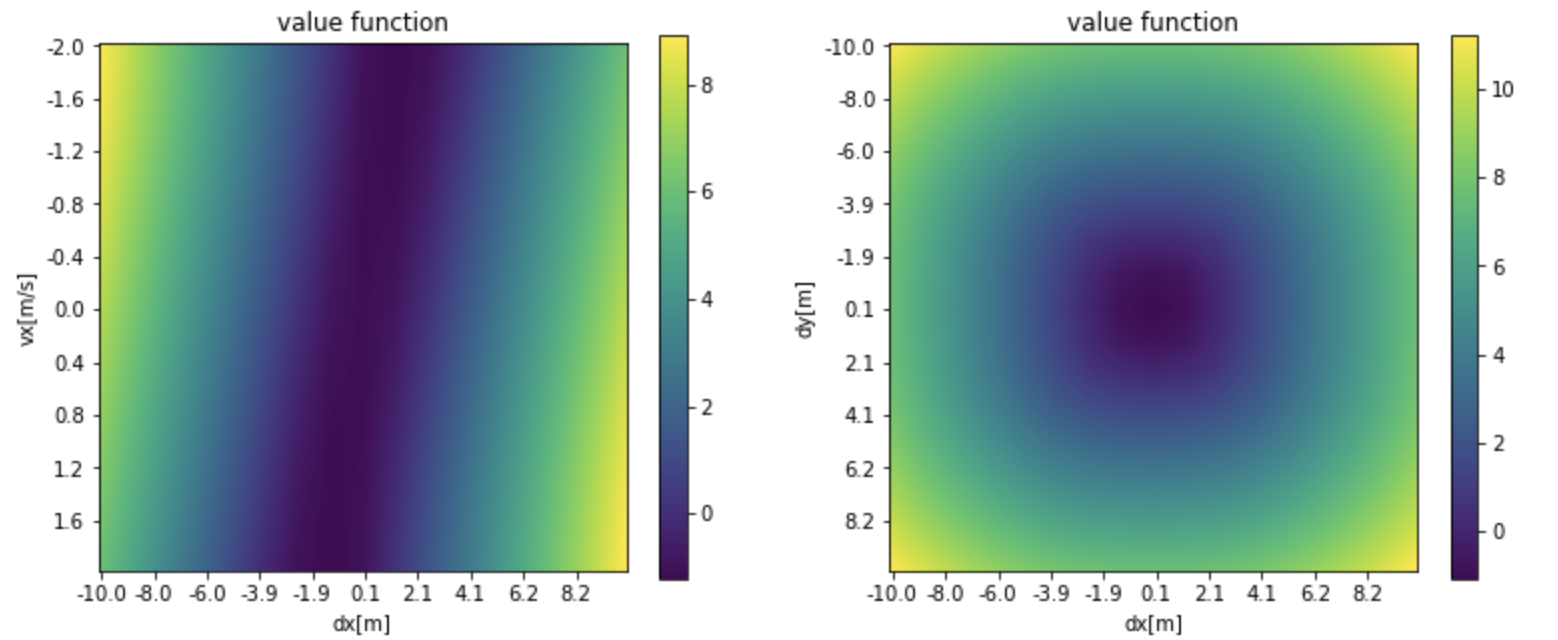
\includegraphics[width=\imgwidth]{images/hj_value_function.png}
\caption{2D slices of 4D \ac{HJR} value function: Position and velocity for one-dimensional case ($y = v_y = 0$, left) and two-dimensional static case ($v_x = v_y = 0$, right)}
\label{img:hj_value_function}
\end{center}
\end{figure}

\subsubsection{Value Function approximation}
Due to the curse of dimensionality the value function cannot be determined with a resolution smaller than $0.5 m$ or $0.5 m/s$, with a feasible amount of pre-computation as well as size of the buffered value function grid and its gradients  on the RAM online \cite{Pavone2020}. There have been several methods for  approximating the value function in post-computation, such as \cite{Zhong2013} comparing the approximate performance of several regression classes such as nearest neighbor or locally weighted projection regression (LMDP) or \cite{Kuper2018} about verifiable safety-critical deep networks. It turns out that using nearest neighbor already lowers the control cost and improves stabilization capability of the value function based MPC control system for diverse (simple) experimental setups such as inverted pendulum, which holds even for time horizons $> 1.5s$. These results motivated comparing several interpolation methods for approximating the value function locally.

\begin{figure}[!ht]
\begin{center}
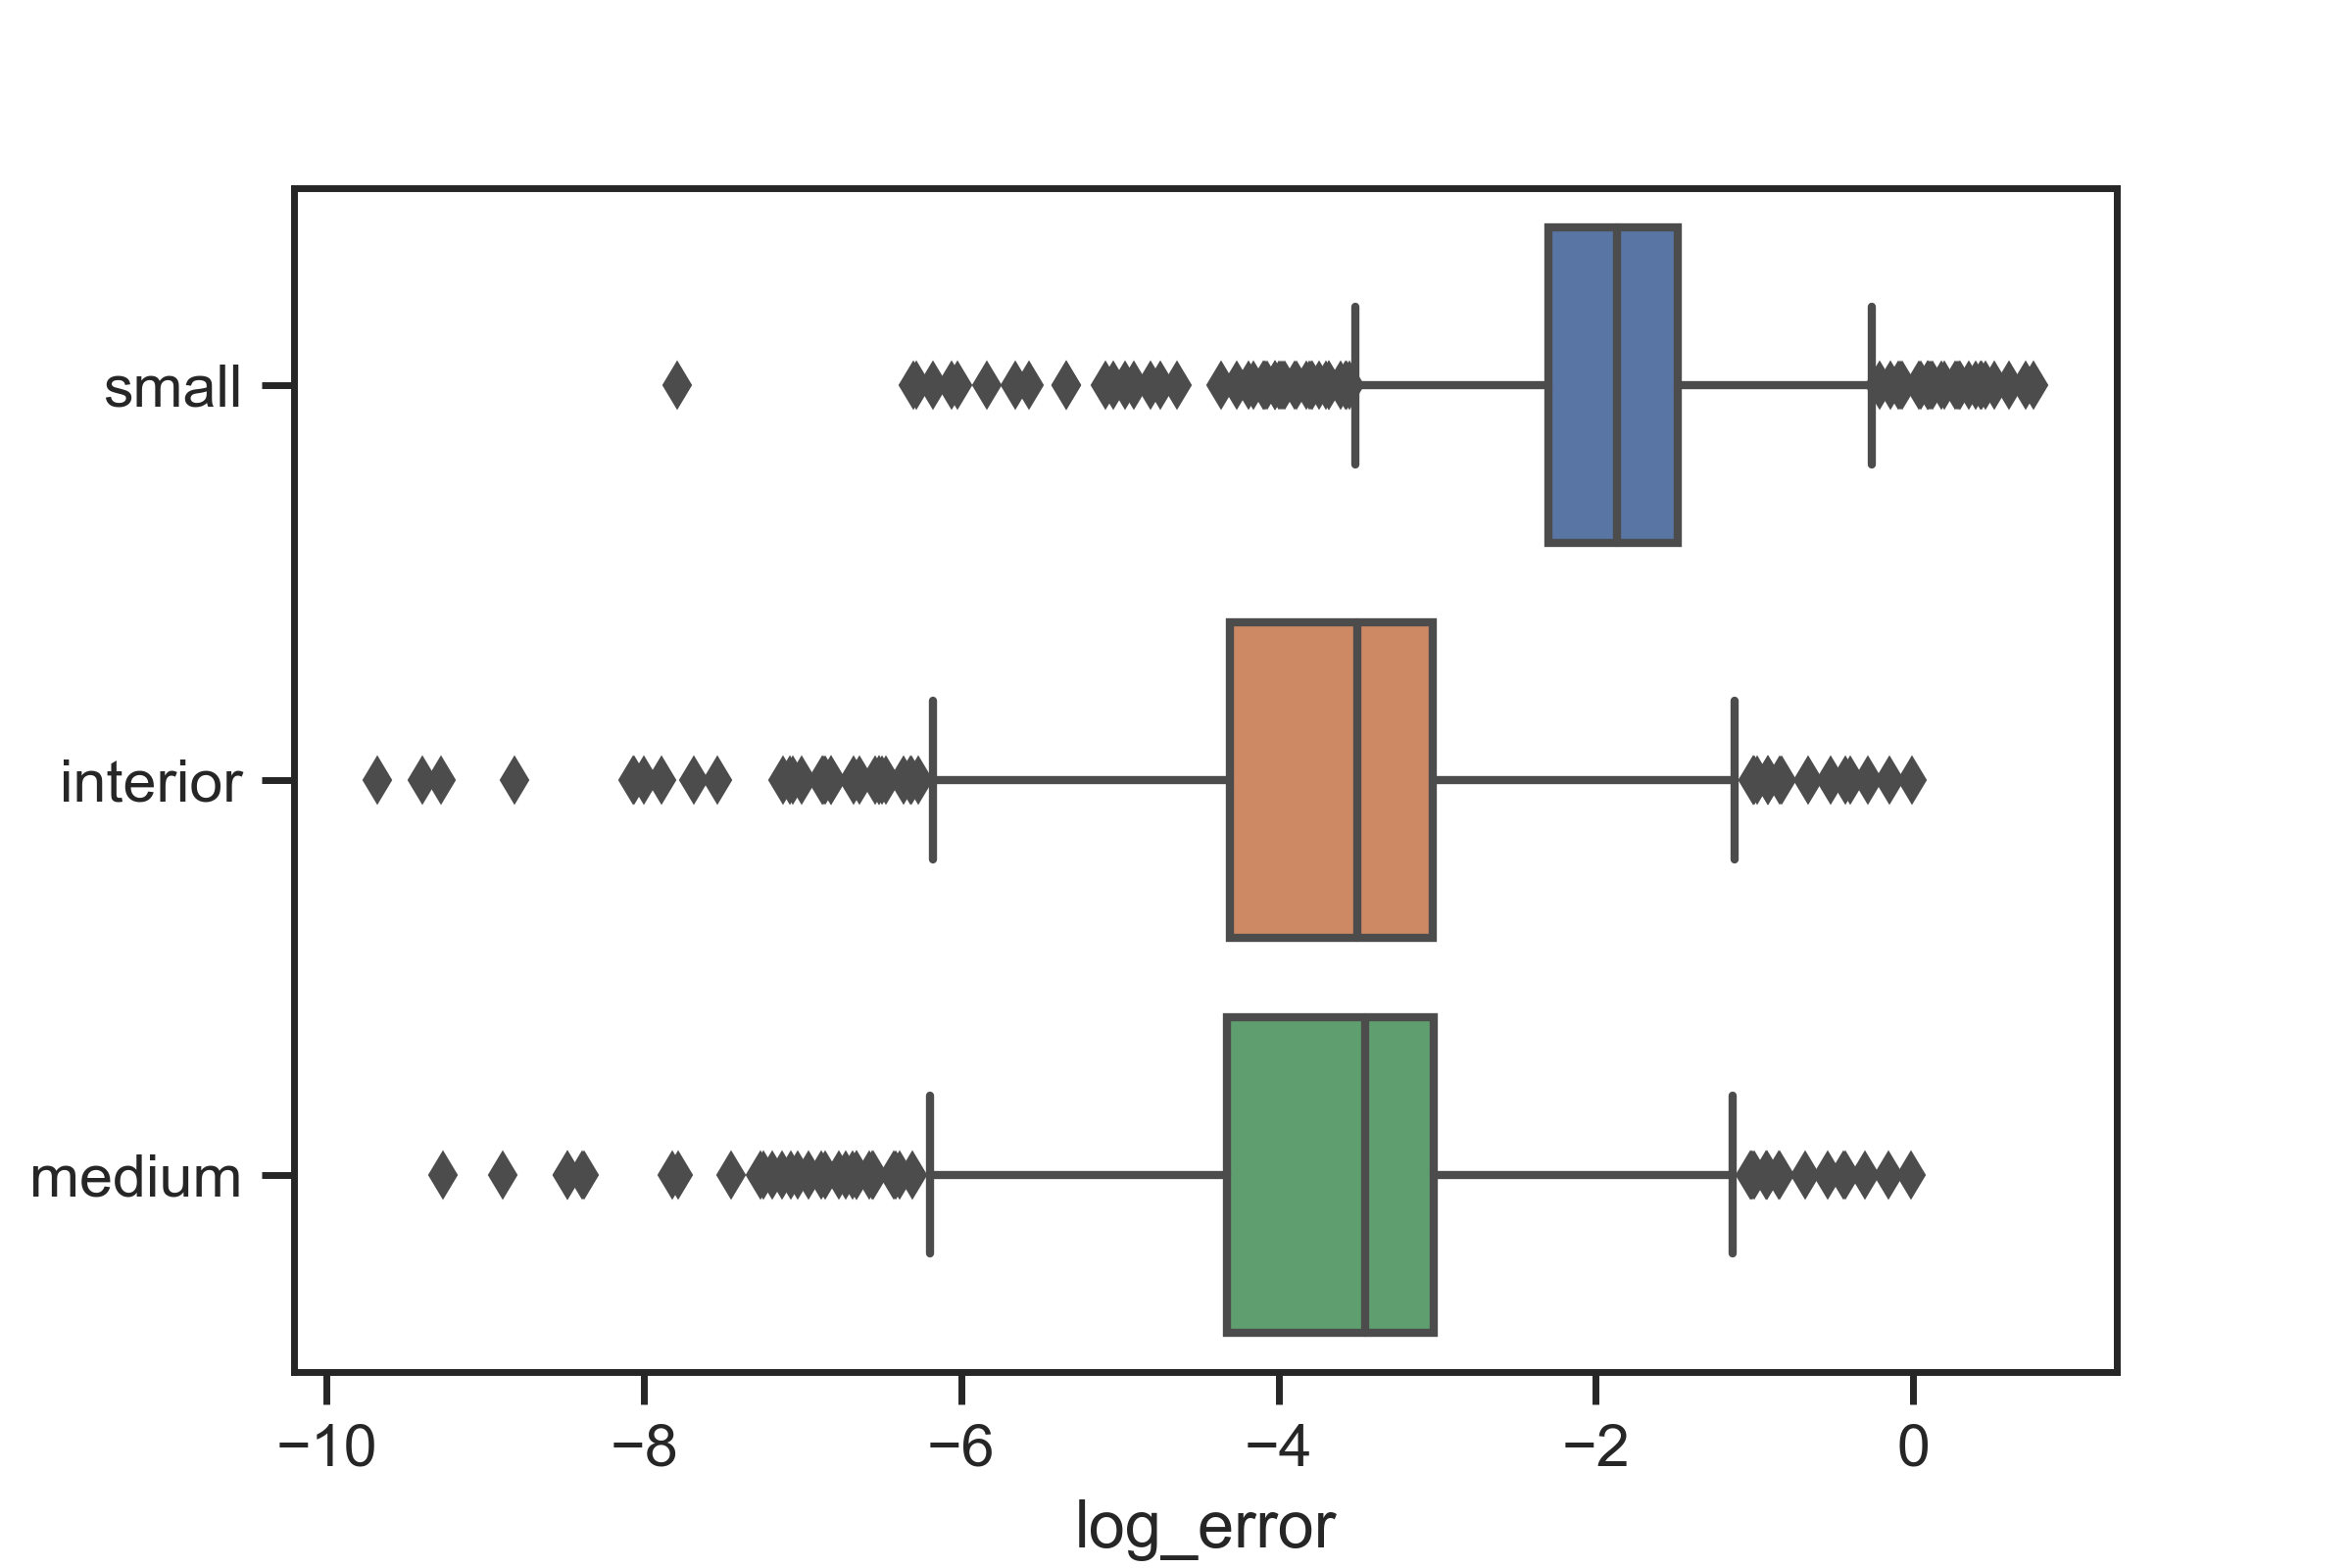
\includegraphics[width=0.45\textwidth]{images/hj_bar_linear.png}
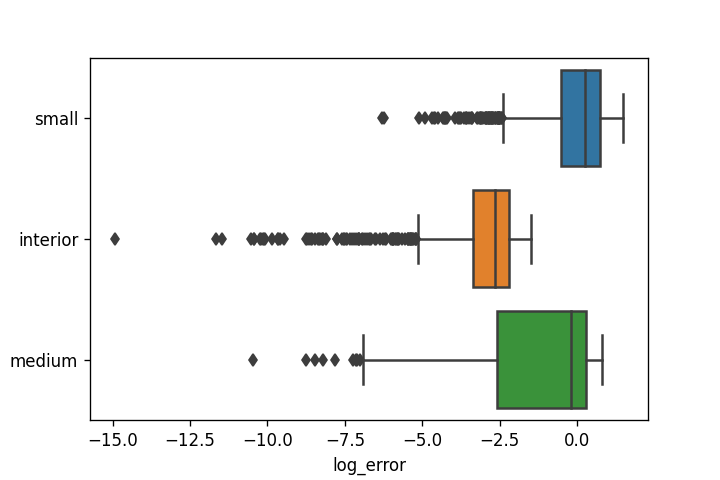
\includegraphics[width=0.45\textwidth]{images/hj_bar_nearest.png}
\caption{Logarithmic value function approximation error using linear (left) and nearest neighbor (right) interpolation methods based on various pre-computed grid sizes (small < interior < medium)}
\label{img:hj_approx_bar}
\end{center}
\end{figure}

\begin{figure}[!ht]
\begin{center}
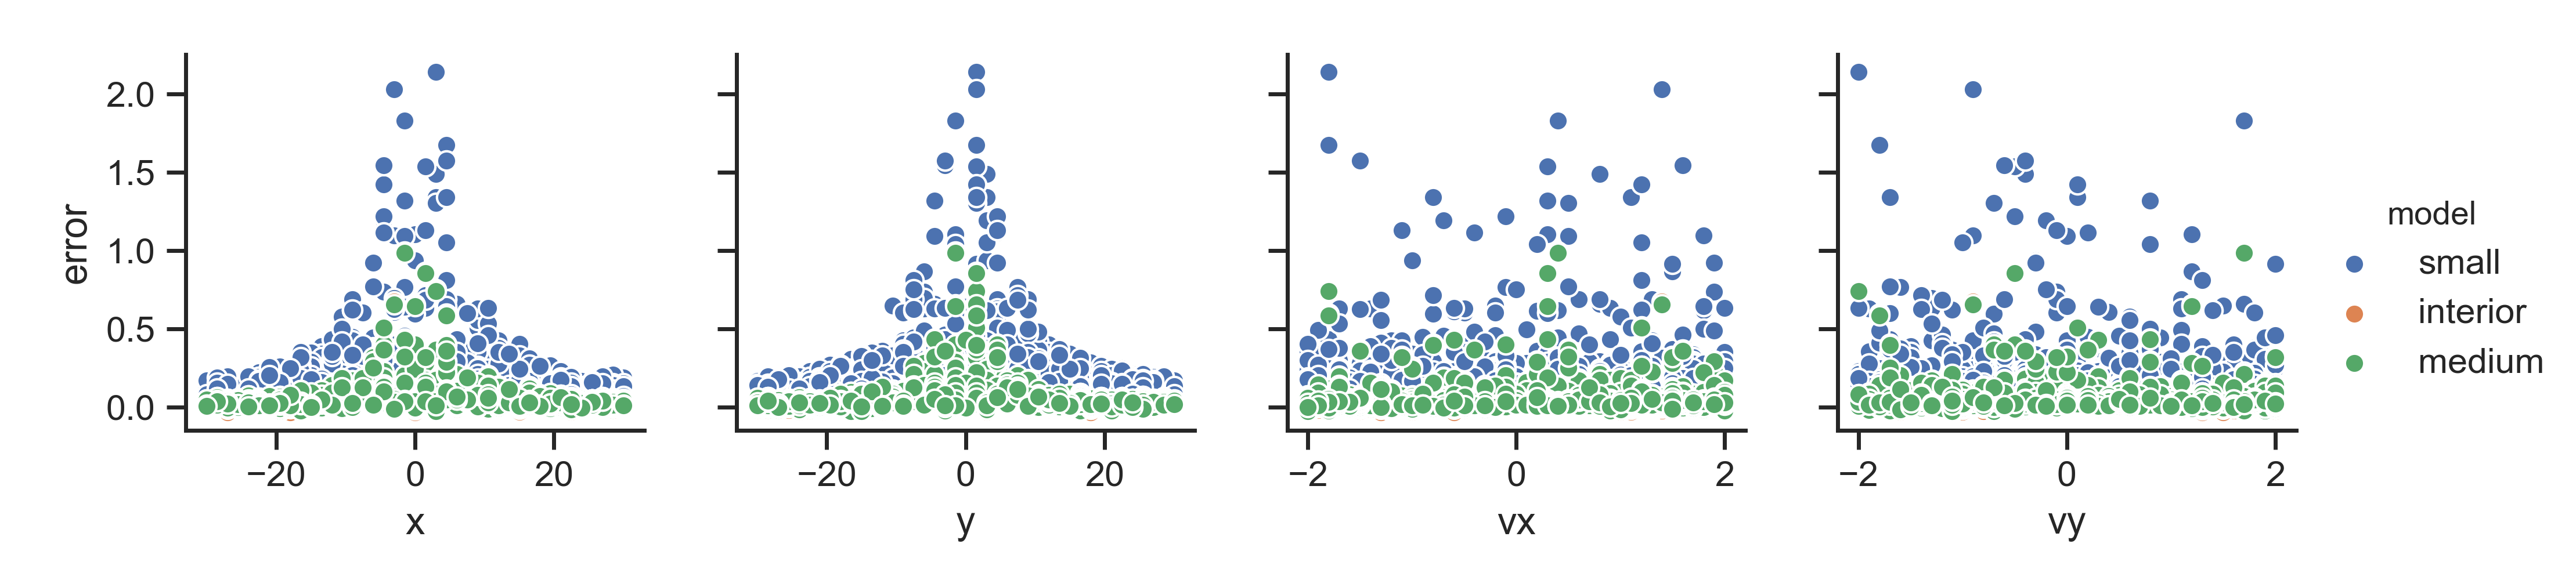
\includegraphics[width=\imgwidth]{images/hj_hist_linear.png}
\caption{Absolute error distribution over joint system state axes using linear interpolation based on various pre-computed grid sizes (small < interior < medium)}
\label{img:hj_approx_hist}
\end{center}
\end{figure}

Figure \ref{img:hj_approx_bar} shows the logarithmic approximation error for several pre-computed grid sizes and using linear (as in \cite{Leung2020}) and nearest neighbor interpolation methods. LWPR (not shown here) has been tested as well but turned out to be infeasible for a large amount of grid points.\footnote{For more information about the implementation of the LWPR value function approximation see \href{https://github.com/simon-schaefer/HJReachibility}{HJ-Reachability Toolbox} on GitHub.} For computing the error metric the value function has been computed on a dense grid exactly, and point-wise compared with the grid interpolated approximations. While linear interpolation widely outperforms nearest neighbor, as expected, the absolute error is very small. As displayed in Figure \ref{img:hj_approx_hist} the interpolation error is not uniform over all joint state axes, but larger for positional axes (which likely is due to the larger amount of non-linearity in position compared to velocity directions, compare Figure \ref{img:hj_value_function}). Therefore, the number of grid points have not been equally distributed over the axes, but biased to the positional axes (interior), while keeping the overall size of the grid constant. 

\subsubsection{\ac{HJR} safety constraint} 
\cite{Leung2020} presents a safety-constraint, based on the resulting value function's gradient, by defining the set of safety-preserving robot control actions as:

\begin{equation}
\uset_{HJR} (\x_{rel}) = \{ \u: \min_{\boldsymbol{d}} \nabla V (\x_{rel})^T \frel(\x, \boldsymbol{d}) \geq 0 \, | \, \u \in \uset \}
\end{equation}

Since the value function $V$ and its gradient $\nabla V$ are computed offline, the constraint is highly efficient to employ online. As the value function has been computed as backward reachable tube, when starting in a safe set $V > 0$ safety is guaranteed for feasible control actions, over the whole time-horizon $T_{HRJ}$, the value function was computed on. Especially, the constraint only depends on the current state, not on future states. Especially the last property make an \ac{HJR}-based constraint very well-suited for project \project. As previously stated evaluating as well as in particular backward passing through the prediction model is the optimization's computational bottleneck. An \ac{HJR}-based safety constraint as described above is however independent from the prediction model. 
\newline
In opposite to \cite{Leung2020} the value function for the joint robot-pedestrian system is negative almost everywhere (comp. Equation \ref{eq:hj_value_negative}), so that a safety-preserving constraint would be infeasible not matter which action is chosen. Therefore the value function itself is bounded, not pre-serving safety but guarantee to stay safe ($\Vrel \leq 0$).

\begin{equation}
\uset_{HJR} (\xrel) = \{ \u: \min_{\dxped[]} \Vrel(\x_{rel} + \frel(\x, \xped[], \u, \dxped[]) \geq \epsilon  \, | \, \u \in \uset \}
\label{eq:hj_constraint}
\end{equation}

To compute \ref{eq:hj_constraint} the value function for all possible pedestrian actions $\dxped[k]$ is determined, conditioned on the current relative state and the chosen robot's control action $\u$. The minimal value with respect to $\dxped[k]$, which reflects the value function in case of the worst-case scenario, given the robot's action, is constrained to be greater or equal zero. If $\u$ in $\uset_{HJR}$ then the robot is guaranteed to be safe from getting close to the pedestrian $k$ within the \ac{HJR}-time-horizon $T_{HJR} = 1s$. Additionally, the buffer $\epsilon > 0$ takes account for interpolation errors. 
\newline
In general it might occur that the relative state itself is infeasible, i.e. has a value term smaller than zero. Due to the inequality \ref{eq:hj_value_negative} there is no control action, that can be chosen by the robot, to reach a positive value. To avoid problem infeasibility, the constraint is appended by a slack variable $\eta \leq 0$, which is strongly weighted in the objective function. 

\begin{equation}
\uset_{HJR} (\xrel) = \{ \u: \min_{\dxped[]} \Vrel(\x_{rel} + \frel(\x, \xped[], \u, \dxped[]) + \eta \geq \epsilon  \, | \, \u \in \uset \}
\end{equation}

\subsubsection{\ac{HJR} multi-agent coupling}
In reality, 

\begin{figure}[!ht]
\begin{center}
\begin{tikzpicture}

    \node[inner sep=0pt] (ped1) at (5,1)
    {
\includegraphics[width=.03\textwidth]{images/walking.png}};
    \fill[orange, opacity=0.3] (ped1) circle (1);
    \draw[dashed, ->] (ped1) to (4, 0);
    
    \node[inner sep=0pt] (ped2) at (-3,-1)
    {
\includegraphics[width=.03\textwidth]{images/walking.png}};
    \fill[orange, opacity=0.3] (ped2) circle (1);
    \draw[dashed, ->] (ped2) to (-1, 0);
    
    \node[inner sep=0pt] (ped3) at (0,2)
    {
\includegraphics[width=.03\textwidth]{images/walking.png}};
    \fill[orange, opacity=0.3] (ped3) circle (1);
    \draw[dashed, ->] (ped3) to (-1, 1);
    
    \node[inner sep=0pt] (ped4) at (2,-1)
    {
\includegraphics[width=.03\textwidth]{images/walking.png}};
    \fill[orange, opacity=0.3] (ped4) circle (1);
    \draw[dashed, ->] (ped4) to (1, -1);
    
    \node[inner sep=0pt] (robot) at (-0.5,0)
    {
\includegraphics[width=.04\textwidth]{images/robot.png}};
    
    \draw [thick] (robot) to[out=0, in=180] (5,3) to[out=0, in=180] node[above, sloped] {$\Vrel \geq 0$ ??} (10, 1);  
    
\end{tikzpicture}
\end{center}
\caption{Avoid set for static ($\dxped[]_t = 0$), single pedestrian scenario}
\label{img:hj_game_multiagent}
\end{figure}



%The system dynamics f : Z ×U → Z is assumed to be uniformly continuous, bounded, and Lipschitz continuous in z for fixed u. 
% any finite number of subsystems defined in the analogous way; however, for clarity and without loss of generality, in this paper we will assume that there are two subsystems.
% intuitively (12) means that the evolution of states in each subsystem depend only on the states in that subsystem: for example, the evolution of x1 depends only on the states in x1. However, the two subsystems are coupled through the state partition y3. 
% Although there may be common or overlapping states in x1 and x2, the evolution of each subsystem does not depend on the other explicitly. In fact, if we for example entirely ignore the subsystem x2, the evolution of the subsystem x1 is well-defined and can be considered a full system on its own; hence, each subsystem is self-contained. ==> each pedestrian plays its own catch-run game, independent from the actions of the other agents
% where the full unsafe set is the intersection of the back projections of subsystem unsafe sets.
% We assume that the full system unsafe set L can be written in terms of the subsystem unsafe sets Lx1 ∈ X1,Lx2 ∈ X2 in the way depicted in Fig. 3:
% Specifically, we will show that if the unsafe set can be decomposed in the way described by (21), then the full-dimensional BRS is decomposable in the same way:


\section{Runtime optimization}
\label{text:approach/runtime}
\subsection{Efficient Trajectory Unrolling}
\label{text:approach/runtime/unrolling}
One of the most promising directions for decreasing the runtime of a trajectory optimization algorithm is to decrease the runtime of the objective and constraints evaluation as well as their gradients. As shown in sections \ref{text:approach/objective} and \ref{text:approach/constraint}, the majority of these optimization modules depend on the robot's trajectory $\x_{0:T}$, rather than on its control inputs $\u_{0:T}$. However, since control inputs are optimized, as described in Section \ref{text:approach/overview}, a computationally efficient transformation from controls and initial state to the trajectory is key for making the trajectory optimization real-time feasible.
\newline
Fortunately, we assumed that the robot follows double integrator dynamics, which are linear and markovian. Hence, they can be expressed as the following: 

\begin{equation}
\x_{t+1} = A \x_t + B \u_t
\label{eq:dynamics}
\end{equation}

\begin{minipage}{0.5\textwidth}
$$A = \begin{bmatrix} 1 & 0 & \dt & 0 \\ 0 & 1 & 0 & \dt \\ 0 & 0 & 1 & 0 \\ 0 & 0 & 0 & 1\end{bmatrix}$$
\end{minipage}
\begin{minipage}{0.5\textwidth}
$$B = \begin{bmatrix} 0 & 0 & \dt & 0 \\ 0 & 0 & 0 & \dt \end{bmatrix}$$
\end{minipage}

Due to the linear (not linearized !) dynamics $\dt = \Delta t$ can be safely used. To fully "unroll" a trajectory, the linear dynamic equation \ref{eq:dynamics} would be applied iteratively for the length of the trajectory. Since the dynamics themselves are linear (not just a first-order approximation), this computation can be further batched and, in this way, speed up. In fact, the full trajectory can be derived merely based on the initial state $\x_0$ and the control input matrix $\u_{0:T}$, as shown in the following:

\begin{align}
\x_1 &= A \x_0 + B \ u_0 \\
\x_2 &= A \x_0 + B \ u_1 = A^2 \x_0 + A B \ u_0 + B \ u_1\\
\hdots &= \hdots \\
\begin{bmatrix} \x_1 \\ \x_2 \\ \vdots \\ \x_n \end{bmatrix} &= \underbrace{\begin{bmatrix} A \\ A^2 \\ \vdots \\ A^n \end{bmatrix}}_{\substack{A_n}} \x_0 + \underbrace{\begin{bmatrix} B & 0 & \hdots & \hdots & 0 \\ AB & B & 0 & \hdots & 0 \\ \hdots & \hdots & \hdots & \hdots & \hdots \\ A^{n-1} B & A^{n-2} B & \hdots & \hdots & B \end{bmatrix}}_{\substack{B_n}} \begin{bmatrix} \u_0 \\ \u_1 \\ \vdots \\ \u_{n-1} \end{bmatrix}
\end{align}

In summary, we get the following (also linear) expression for computing the full robot trajectory at once. As demonstrated in \href{https://github.com/simon-schaefer/mantrap/blob/master/examples/timing.ipynb}{examples/tools/timing} using the fully batched formulation speeds up the trajectory "unrolling" by about a factor of 30.

\begin{equation}
\x_{1:n} = A_n \x_0 + B_n \u_{0:T-1}
\label{eq:dynamics_stacked}
\end{equation}

\subsection{Warm Starting}
\label{text:approach/runtime/warm_starting}
It is widely known that warm starting an optimization can be very beneficial for its convergence speed for several optimization algorithms, e.g. shown in \cite{Banerjee2020} for \ac{GuSTO} or for \ac{IPOPT} in \cite{Shahzad2010}, \cite{John2008} or \cite{Spielberge2019}.
\newline
Within project \project the algorithm has been warm-started by solving the optimization problem posed in problem \ref{eq:formulation} while ignoring all objectives and constraints that relate to pedestrians, i.e. by solving the following optimization problem: \\

\begin{problem}{Simplified optimization problem for warm-starting}
\begin{align}
\min_{\u_{0:T-1}} \quad & J_{goal}(\x_{0:T}) \\
\textrm{s.t. } \quad & \x_{t+1} = \f(\x_t, \u_t) & \forall t \in [0, T - 1] \\
& \x \in \xset & \forall t \in [0, T]\\
& \u_t \in \uset & \forall t \in [0, T]\\
& \x_0 \in \xset_0
\end{align} 
\label{eq:formulation_warm_starting}
\end{problem}

Since the simplified optimization problem in problem \ref{eq:formulation_warm_starting} does not depend on the pedestrian dynamics model $\tilde{\Phi}$ it is much easier and more efficient to solve, being a convex quadratic program. \\

\begin{figure}[!ht]
\begin{center}
\begin{tikzpicture}

    \node (R) at (0, 0) [circle, shade, draw] {Robot};
    \node (G) at (8, 4) [circle, shade, draw] {Goal};
    \node (P1) at (2, 3) [circle, fill=orange, draw] {$P_1$};
    \node (P2) at (8, 1) [circle, fill=yellow, draw] {$P_2$};
    
    \tkzDefPointBy[projection=onto R--G](P1)  \tkzGetPoint{P1m}
    \tkzDefPointBy[projection=onto R--G](P2)  \tkzGetPoint{P2m}
    
    \draw[->, dotted, very thick] (R) to node[above] {} (G);
    \draw (P1m) -- (P1) node[midway, sloped, above] {$\mu_{P1}$};
    \draw (R) -- (P1m) node[midway, sloped, above] {$\eta_{P1}$};
    \draw (P2m) -- (P2) node[midway, sloped, above] {$\mu_{P2}$};
    \draw (R) -- (P2m) node[midway, sloped, below] {$\eta_{P1}$};
    
\end{tikzpicture}
\end{center}
\label{img:robot_goal_encoding}
\end{figure}

%Does the pre-computed set contain every possible scenario? No, but just warm-start so not required, there will be a constrained optimization afterward anyway

\subsection{Attention}
\label{text:approach/runtime/filtering}
For a trajectory optimization to be feasible for online applications, it must be efficient to solve. As empirically shown by experiments in Section \ref{text:experiments/unit}, the computational bottleneck of solving Problem \ref{problem:general} is evaluating and, particularly, differentiating the components, which depend on the interaction between robot and pedestrians. By design, the computational cost of the safety constraint has already been reduced. However, the interactive cost presented in Section \ref{text:approach/objective/interactive} cannot be further runtime optimized or occluded, being one of the core parts of the underlying algorithm. Therefore there are mostly two ways to increase overall runtime efficiency of the trajectory optimization: Firstly, reducing the number of solver iterations for convergence and secondly lowering the runtime cost of evaluating the optimization components itself.
\newline
While the number of solver iterations has already largely been reduced by warm-starting the optimization, the attention focusses on merely taking into account essential factors into the evaluation, with improves runtime without having a significant impact on the resulting behavior of the algorithm. Accurately, the attention filter decides which pedestrians are taken into account for a specific (interactive objective) function evaluation. Importantly to note here, that attention merely effects the evaluation of the interactive objective function (including its gradient computation). Especially, it is not applied to the safety-relevant constraints, to guarantee safety regarding all pedestrians at every time.    
\newline
Using the distance between the robot as each pedestrian is a natural choice for filtering out the agents to consider for the trajectory optimization; the larger the distance is, the smaller the impact of the robot probably is. In fact, the Trajectron model uses a similar distance-based metric for building and evaluating edges in their graph network \cite{Salzmann2020}.

\begin{equation}
\attention(\x, \xped[k]) = \left( ||\x - \xped[k]||_2 > D_{Attention} \right)
\end{equation}

Although euclidean distance-based filtering is a quite naive way of distributing attention to pedestrians in the scene, it shows to be quite effective in reducing the runtime of the interactive objective and gradient evaluations, and therefore of the whole algorithm. A comparison to more sophisticated approaches such as using (forward) reachability to conservatively estimate the pedestrians that eventually could impinge on the robot trajectory, or focussing on only a specific pedestrian instead of a set of pedestrians, as used by game-theoretic crowd navigation works (as presented in Chapter \ref{text:related/crowd_navigation}, e.g.\,  \cite{Bouzat2014}\cite{Nikolaidis2017}), is given in Section \ref{text:experiments/unit}.


\chapter{Experiments and Results}
\label{text:experiments}

\section{Simulation Environments}
\label{text:experiments/environments}

\section{Baselines}
\label{text:experiments/baselines}

\section{Experimental Results}
\label{text:experiments/results}
\chapter{Conclusion and Future Work}
\label{text:conclusion}

\section{Conclusion}
\label{text:conclusions/conclusions}
In this thesis, I designed and implemented a new approach of socially-aware trajectory optimization for crowd-navigation. In this field, purely data-driven methods lack tractability, while model-driven systems usually miss the predictive power of learned generative models. The purposed optimization formulation combines the strengths of both methodologies and is seamlessly integrating into probabilistic, multi-model, state-of-the-art prediction models. Thereby, it harnesses its predicted distributions over future pedestrian states precisely and without the need for sampling methods.
\newline\newline
By directly leveraging the prediction model's internal structure, the interactive objective function drives the optimization to (socially) anticipative but cautious solutions. An \ac{HJR}-based constraint further guarantees interaction safety within the planning horizon, without being overly conservative.
\newline\newline
Several strategies have been substantiated and implemented to efficiently solve the designed optimization using the interior-point method-based solver \ac{IPOPT}.
\newline\newline
Finally, I presented results and validated the final algorithm for an assorted set of pedestrian prediction models in simulation. A sampled-based algorithm has been proposed to compute an output distribution for deterministic, parametric models. In comparison to other state-of-the-art, both data-driven as well as conventional trajectory planning algorithms, the purposed approach shows great performance.
\newline

\section{Future Work}
\label{text:conclusions/future_work}
In the following, I list possible extensions and future research directions.

\begin{itemize}
\item For fully integrating the purposed planning methodology into real-world applications, several external determinants have to be considered in planning. While undoubtedly the most challenging factor, the interaction with dynamic agents, has been treated within this work, integrating the structure of the environment itself (such as sidewalks, roads, static-obstacles), remains for future work. Since most prediction models such as Trajectron \cite{Salzmann2020} do already support including the environment structure, doing so probably is straight-forward. As previously shown, most data-driven prediction models have been trained on data recorded in structured environments, leading to (unintentional) artifacts in their prediction. Adding structure to the environment, therefore, may even improve the performance of the overall approach.
\item The bottleneck of the purposed approach is the number of evaluations of the interactive objective and its gradient. \ac{SQP} has shown to require less objective function evaluations compared to interior-point methods, at the cost of intermediate infeasibility. To further improve the algorithm's efficiency, it might be reasonable to use a \ac{SQP}-based solver such as Gusto \cite{Bonalli2019} instead.
\item Due to the lack of robot-conditioned prediction models, the algorithm could only be validated for a selected set of models. A future research direction may condition other state-of-the-art pedestrian prediction models on the planned robot's trajectory, such as \ac{SGAN} \cite{Gupta2018}, and integrate these into the planning framework. This includes evaluating the framework on other "socially-aware" agent types, such as bicyclists or cars. Therefore, in theory, no non-parametric change in the overall formulation is required.
\item During this work, it is assumed for the robot to underly double integrator dynamics. A generalization of the method to other robot dynamics should be straight-forward.
\item Finally, the algorithm has been tested in simulation only, mainly due to the implications of COVID-19. While several efforts have been introduced to mimic the challenges of a real-world environment as best as possible, they obviously could not perfectly be matched. Thus, despite the discussed drawbacks of real-world testing in terms of comparability of the results, it remains for future work to test it in a real-world environment. 
\end{itemize}

The interactive optimization design fully leveraging the predictive power of a learned deep neural network has never been done before for trajectory optimization, to the best of my knowledge. With the rise of data-driven prediction models, it gains increasing importance to unleash their full predictive power in optimization in many fields. Therefore, this work can be seen as a proof-of-concept of applying this concept in trajectory optimization and many other optimization-driven fields, such as adaptive control or manufacturing optimization. In contrast to purely learning-based approaches using online optimization gives rise to the possibility of constraint the solution in a tractable manner. Due to the ongoing trend of neural network compression in many fields, computational bounds of the purposed approach will fade. With an increasing amount of computational complex simulation being replaced with data-driven approaches, this work may be one of the foundations for applying neural network gradients in online optimization.

\appendix
\chapter{Appendix - Math Prerequisites}

\section{GMM Log Probability Value}
\label{appendix:gmm_log_prob}
For a two-dimensional \ac{GMM} $g \sim GMM(\mu, \Sigma, \pi, \rho)$ with mean vector $\mu$, variance matrix $\Sigma$, mode importance vector $\pi$ and Pearson's correlation coefficients $\rho$ the probability at $(x, y)$ can be computed as:\footnote{\href{https://de.wikipedia.org/wiki/Mehrdimensionale_Normalverteilung}{Wikipedia - Multivariate Normal Distribution}}.

\begin{align}
f_m(x, y | \mu, \sigma, \rho) 
&= \frac{1}{2 \pi \sqrt{\det \Sigma}} \exp \left(- \frac{1}{2} (\boldsymbol{x} - \boldsymbol{\mu})^T \Sigma (\boldsymbol{x} - \boldsymbol{\mu}) \right) \\
&= {\frac{\sqrt{1- \rho^2}}{2 \pi \sigma_x \sigma_y} 
\exp - \frac{1}{2 (1 - \rho^2)}} \left( \frac{( x - \mu _x)^2}{\sigma_x^2} +
\frac {(y - \mu_y)^2}{\sigma_y^2}-{\frac {2\rho (x - \mu_x)(y - \mu_y)}
{\sigma_x \sigma_y}} \right)	
\end{align}

The Pearson coefficient is the covariance for two normalized random variables $X$ and $Y$, in their normalized form $\tilde{X} = (X - \mu_x)/\sigma_x$ and $\tilde{Y} = (Y - \mu_y) / \sigma_y$. Using the law of linear transformations of covariances we get:\footnote{\href{https://en.wikipedia.org/wiki/Pearson_correlation_coefficient}{Wikipedia - Pearson correlation coefficient}} 

\begin{equation}
Cov(\tilde{X}, \tilde{Y}) = \frac{1}{\sigma_x \sigma_y} Cov(X, Y) = \rho_{X, Y}
\end{equation}

The expected value over all modes $m \in [0, M]$ super-imposes the \ac{PDF} for the bi-variate Gaussian distributions, weighting each one by its importance $\pi_m$:

\begin{equation}
\mathbb{E}_{GMM}[x, y] = \sum_{m=0}^M \pi_m \cdot f_m(x, y) =  \sum_{m=0}^M \exp \left( \log \pi_m + \log f_m(x, y) \right)	
\end{equation}


%\begin{figure}[ht!]
%\begin{center}
%\begin{tikzpicture}[node distance=1cm, auto,]
%
%\node[rectangle, rounded corners, draw=black, very thick, text width=8.5em,
%      minimum height=2em, text centered](intermediate) {Pedestrian States\\$\muped[j]_t, \sigmaped[j]_t$};
%\node[rectangle, rounded corners, draw=black, very thick, text width=8.5em,
%      minimum height=2em, text centered, below=0.5cm of intermediate](robot) {Robot state\\$\x_t$};
%
%\node[above=of intermediate] (dummy) {};
%\node[right=of dummy] (t) {Particle simulation()}
%   edge[<-, bend left=45] (robot.east)
%   edge[<-, bend left=45] (intermediate.east); 
%\node[left=of dummy] (g) {Accumulation()}
%   edge[->, bend right=45] (intermediate.west)
%   edge[<-, bend left=45] (t)
%   edge[<-, bend left=50] (t)
%   edge[<-, bend left=40] (t);
%\end{tikzpicture}
%\end{center}
%\caption{...}
%\label{fig:particle_simulation}
%\end{figure}


%\chapter{Problem Definition}
%\label{chp:problemDefinition}
%In this work, we are interested in deriving a trajectory planning algorithm based on the Trajectron behavioral prediction model \cite{Ivanovic18}. The Trajectron combines elements of variational deep generative models (\ac{VAE}), recurrent sequence models (\ac{LSTM}) and dynamic spatio-temporal graphical structures to predict the possible movements, i.e. velocity distributions, of each agent in a scene, given their state trajectories. 
%
%\begin{figure}[h]
%\centering
%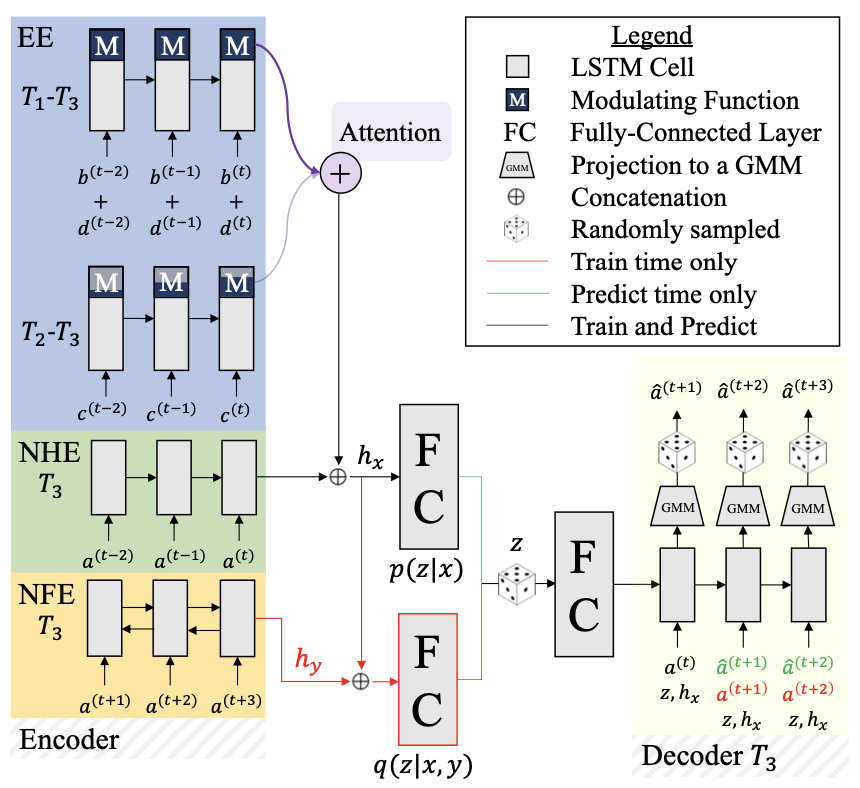
\includegraphics[width=0.5\textwidth]{images/trajectron.png}
%\caption{Trajectron model architecture  \cite{Ivanovic18}}
%\label{fig:trajectron_architecture}
%\end{figure}
%
%The architecture of Trajectron is shown in Fig. \ref{fig:trajectron_architecture}. First the history of each agent (node) is as well as their relations between each other (edges) are encoded, added and transformed to a discrete latent space $z$. By random sampling from $z$ the future velocity distributions are predicted iteratively. In order to approximate a multi-modal, general distribution for every time-step a \ac{GMM} is used. While unrolling the For each $0 < t < T$ in the prediction horizon a sample is drawn from the previously predicted distribution and inputted in the next \ac{LSTM} cell. Therefore, the velocity distribution of each agent in the scene for $t > 1$ is modelled as a nested \ac{GMM} distribution (the velocity distribution at $t = 0$ is a \ac{GMM}). 
%\newline
%In general a planning algorithm that determines a trajectory that is risk-aware of colliding with another agent based on the behavior predictions of the Trajectron model has to deal with multi-modal and time-evolving risk efficiently. Since each distribution depends on the full state history, not on the last state only, the transitions are a \ac{POMDP} (given that not the full history is part of the state vector). For simplicity we assume the ego's dynamics to be known and deterministic. Formally speaking we want to optimize a given cost function $J(x(t), u(t))$ while being constrained by some collision risk threshold $R_{max}$: 
%
%\begin{equation}
%\begin{aligned}
%\min_{x(t), u(t)} \quad & J(x(t), u(t)) = \sum_{k = 0}^{N-1} l(x_k, u_k) + l_f(x_N) \\
%\textrm{subject to} \quad & x_{k + 1} = f_{ego}(x_k, u_k) \\
%    &x_0 = x(0) \\
%    &x_N = x_{goal} \\
%    &\sum_{k = 0}^N r(x_k, u_k) \leq R_{max} \\
%\end{aligned}
%\end{equation}
%
%
%\chapter{Related Approaches}
%\label{chp:AppendixRelatedApproaches}
%
%\begin{itemize}
%    \item Chance-Constrained Model Predictive Control \cite{Lew2019}, \cite{Ono2015CCMPC}, \cite{Ono2012}, \cite{Blackmore2012}, \cite{chow2015DTRC}, \cite{ono2008}: CCMPC minimizes the cost function $J(x(t), u(t))$ with respect to a point-wise risk allocation constraint. Therefore the solution is guaranteed to be first-order and locally optimal (comp. \cite{bonalli2019}) and to fulfill the risk constraint, instead of deriving some trade-off between risk and cost (when the risk would be part of the cost function). However the constrained risk distribution is neither convex nor linear, therefore it cannot be used directly in a constraint (efficiently), but has to be reformulated as following (re-approximate in every step, SQP). To reformulate these constraints the distribution has to be remodelled in "analytically" expressible distributions: 
%    
%    \begin{itemize}
%        \item Mean-variance analysis ("ellipsoidal" overlapping) \cite{herzog2006}, \cite{hewing2018}, \cite{Lew2019} (when $y ~ N(\mu, \Sigma)$ and $\chi = $ quantile of chi-squared distribution): 
%        
%        $$Pr(||x - y||_2 \geq r) \geq \rho_{max}$$ $$||x-\mu||_2 + \lambda_{max}(\sigma) * \chi(\rho_{max}) \geq r$$
%        
%        \item Cone Constraint (\cite{calafiore2006}, \cite{Lew2019})
%    \end{itemize}
%    
%    Following \cite{ono2008} the risk allocation and the control sequence with tightened constrained can be divided in two steps (iterative risk allocation), in order to be less conservative in estimating the real risk and more computationally efficient.
%    
%    \item Belief Space Planning using Sequential Action Control \cite{ansari2017}, \cite{nishimura2019}: Given some nominal trajectory (e.g. just going straight from start to goal position) find the optimal perturbation for optimizing control objective (J = Tracking + Control + RBF for risk, entropy risk, risk-awareness of ego is controlled by $\sigma$-factor in risk-related control objective) by forward simulation and backward derivation of Hamiltonian.
%    
%    \item Chance-Constrained Rapidly-Exploring Random Trees \cite{Luders2011}, \cite{Luders2010}, \cite{Luders2013}, \cite{Aoude2013}: Under the assumption of linear Gaussian systems RRT can be used for chance-constrained trajectory optimization in continuous space by propagating both the mean and the variance of a state. CC-RRTstar guarantees asymptotic optimality, while a particle based approach can be used for non-linear system dynamics. As shown in \cite{Aoude2013} this approach can be used for dynamic and uncertain obstacles such as pedestrians. While not being applicable to "proper" real-time learned sampling distributions can be used to speed up convergence \cite{Ichter2017}.
%    
%    \begin{figure}[H]
%    \centering
%    \includegraphics[width=0.4\textwidth]{images/rrtcc_loop.png}
%    \includegraphics[width=0.4\textwidth]{images/rrtcc_expansion.png}
%    \caption{Chance-constrained RRT algorithm \cite{Luders2013}}
%    \label{fig:rrtcc}
%    \end{figure}
%  
%    \item Multi-Policy Decision-Making \cite{Galceran2017}: Based on a set of (pre-computed) policies first match the observed behavior of each agent to some policy (Baysian changepoint detection), then sample from policy in order to obtain high-likelihood action for each agent. Afterwards forward simulate all assigned policies and execute the policy with maximum expected reward value. 
%    
%    \begin{figure}[H]
%    \centering
%    \includegraphics[width=0.5\textwidth]{images/mulitpolicy_policy_section.png}
%    \caption{Policy selection algorithm \cite{Galceran2017}}
%    \label{fig:mulitpolicy_policy_section}
%    \end{figure}
%    
%    \item Chance-Constrained Dynamic Programming \cite{Ono2015DP}, \cite{chow2015}
%    
%    \item \ac{POMDP} solver (e.g. POMDP-lite \cite{Chen2016} or DESPOT-alpha \cite{Garg2019}): In general the state transitions in the Trajectron model are \ac{POMDP}s. When discretizing states (continuou => particle filter) and actions a policy can be determined that maximizes some human-engineered utility function, given random state transitions as defined by the Trajectron model. Although computationally very expensive, especially it scales badly with increasing space resolution, the solution in theory should be (globally) optimal. Similarly online belief state planning methods such as Monte Carlo tree search (e.g. POMCP \cite{silver2010}), Lookahead with approximate value function, etc. might be used (maybe based on some offline-computed utility function). However the problem's structure is not used that could safe computational expenses. 
%    
%    \item Deep Reinforcement Learning \cite{Chen2017}, \cite{Everett2018}: Socially aware reinforcement learning approach mapping directly from ego's and other agent's joint state to a trajectory: 
%    
%    \begin{align*}
%        s &= \begin{bmatrix} s_{ego} & s_{o} \end{bmatrix} \\
%        s_{ego} &= \begin{bmatrix} d_g& v_{pref} & v_x & v_y & \psi & r  \end{bmatrix} \\
%        s_o &= \begin{bmatrix} \title{p}_x & \title{p}_y & \title{v}_x & \title{v}_y & \tilde{r} & \tilde{d}_a & \title{\phi} & \tilde{b}_{on} \end{bmatrix}
%    \end{align*}
%    
%    while the reward function is a sum of human-engineered encoded social norms (e.g. right-hand rule). 
%    
%    \begin{figure}[H]
%    \centering
%    \includegraphics[width=0.5\textwidth]{images/DRL_socially_aware.png}
%    \caption{DRL update rule \cite{Everett2018}}
%    \label{fig:DRL_socially_aware}
%    \end{figure}
%    
%    \item Safe-Interval Planning \cite{Phillips2011}: Efficient AStar graph search for dynamic obstacles using time-intervals instead of single time-steps for planning, in order to avoid the increase in the dimensionality of the planning problem with increasing time horizon (safe intervals = time-intervals without collision). SIPP provides the same optimality and completeness guarantees as planning with time as an additional dimension (time-steps). For every grid cell the sequence of safe and collision intervals is defined based on a risk-threshold (i.e. point-wise risk allocation). 
%    
%    \item Inverse Reinforcement Learning \cite{Tschiatschek2019}: In order to shrink the search space for finding a trajectory inverse reinforcement learning can be used based on the offline computation of "good" trajectories (e.g. human demonstration, brute-force, DESPOT, etc.) for some scenarios. Thereby the reward function can be built, which basically can be used as a single, static cost-map which can be used by "standard" path planning algorithms such as Dijkstra to find an optimal trajectory. As shown in \cite{Tschiatschek2019} IRL can be used to both match the teacher’s demonstrated behavior but also takes its constraints, such as physical constraints of the ego dynamics or point-wise risk constraints. However a lot of optimal trajectories still are required for training. Compared to mapping from the observations to the policy directly using IRL is more tractable, since the resulting cost map might be interpretable. 
%    
%    \item Adaptive Dimensionality \cite{Vemula2016}
%    
%    \item Signal Temporal Logic \cite{Sadigh2016}
%    
%    \item Optimal Reciprocal Collision Avoidance \cite{Ma2018} \cite{Berg2011} \cite{Hennes2012} \cite{Luo2018}: Local collision avoidance algorithm modeling the pedestrians as velocity obstacles with deterministic (just one or a set of) velocity. To determine the velocity of every agent in the scene for every pair of agents a set $VO_{A|B}^\tau$ (the velocity obstacle for $A$ induced by $B$ for time window $\tau$) is constructed. Using LP the minimal velocity adaption for every agent is determined so that no pair of velocities is in some velocity obstacle set, assuming that all agents follow the same strategy (!). In \cite{Luo2018} ORCA is adapted to model pedestrian movement by e.g. introducing a notion of patience and to deal with non-holonomic dynamics (P-ORCA). Using Hyp-DESPOT in every time-step the belief of the pedestrians intentions is updated (actions = [ACCELERATE, DE- CELERATE, or MAINTAIN] and some human-engineered reward function trading collision and speed of the agent), which is used for a path update (Hybrid Astar) and velocity updates (P-ORCA).  
%
%\end{itemize}
%
%There are several categories from which the properties of planning approaches can be evaluated: 
%
%\begin{itemize}
%    \item Optimality: trajectory cost vs minimal possible (optimal) cost
%    \begin{itemize}
%        \item globally: $J(x(t), u(t)) = J^*(x(t), u(t)) \forall t$
%        \item locally: $J(x(t), u(t)) \approx J^*(x(t), u(t)) \forall x(t) + \epsilon, u(t) + \epsilon $
%        \item not at all
%    \end{itemize}
%    
%    \item Risk-Awareness: Point-wise constraints are easier to fulfill since each state can be regarded individually, however it assumes independence between the states, which is clearly not given due to the dynamical constraints of the ego. As shown in \cite{JansonSP15} both the additive and multiplicative formulation do not scale with increasing planning horizon, since the accumulated risk converges to infinity. Also the using point-wise constraint often is a very conservative choice, as it does not allow to take more risk at some point to be more efficient or to save risk somewhere else. 
%    \begin{itemize}
%        \item trajectory-wise: $\sum_{k = 0}^N r(x_k, u_k) \leq R_{max}$
%        \item point-wise: $r(x_k, u_k) \leq R_{max} \forall k$
%    \end{itemize}
%
%    \item Computational Feasibility:  
%    \begin{itemize}
%        \item real-time planning
%        \item online policy/trajectory correction (e.g. using perturbation) 
%        \item not real-time applicable
%    \end{itemize}
%    
%    \item Explainability/Tractability \& Guarantees: When the result of the planning algorithm is not tractable it is very hard (or even impossible) to give theoretical guarantees with respect to safety constraints. Therefore for these approaches an additional step, determining the empirical risk of collision using Monte Carlo simulations, is necessary, at the cost of additional run-time.  
%\end{itemize}
%
%\begin{center}
%\begin{tabular}{c||p{2cm}|p{1cm}|p{2cm}|p{1cm}|p{1cm}|p{1cm}|p{1cm}|p{1cm}}
%    Method & 
%    \rotatebox[origin=c]{90}{Space ?} &  \rotatebox[origin=c]{90}{Risk-Awareness ?} & 
%    \rotatebox[origin=c]{90}{PPDF Model ?} & 
%    \rotatebox[origin=c]{90}{Risk as cost ?} &
%    \rotatebox[origin=c]{90}{Optimality ?} &
%    \rotatebox[origin=c]{90}{Parametrization ?} &
%    \rotatebox[origin=c]{90}{Interactive ?} &
%    \rotatebox[origin=c]{90}{Tractability ?} \\
%    \hline\hline
%    
%    CCMPC & continuous & point-wise & approximate (uni-Gaussians) & no & locally & sparse & no & yes \\
%    \hline
%    SIPP & discrete & point-wise & accurate (sampled GMM) & no & globally & sparse & no & yes \\
%    \hline
%    DRL & continuous & none & none & no & none & much & yes & no \\
%    \hline
%    PORCA & continuous & none & none & none & none & much & yes & no \\
%    \hline
%    SACBP & continuous & yes & accurate (sampled traject.) & yes & locally & sparse & no & yes \\
%    \hline
%    POMDP & discrete & yes & accurate & yes & globally & much (state definition) & no & yes \\
%    \hline
%    IRL & discrete & yes & accurate & none & none & much (optimal trajectory) & medium & medium
%    
%\end{tabular}
%\end{center}
%
%
%\chapter{Ideas}
%\label{chp:AppendixIdeas}
%
%\section{Planning Approaches}
%\label{sec:planning_approaches}
%
%
%\section{Approximation Approaches}
%\label{sec:approximation_approaches}
%Over a time horizon t > 1 the Trajectron model predicts by sampling from the previously generated distribution. Therefore the distribution of velocities over multiple time-steps is a nested GMM. While samples from the distribution are accessible by iteratively applying the model and can be easily forward integrated (since position-based information are more straight forward to integrate in most planners) getting the distributions themselves is not straight-forward. However it can be approximated: 
%
%\begin{itemize}
%    \item Sample trajectories from the model, integrate them and approximate the obtained distribution 
%    \begin{itemize}
%        \item \ac{GMM}s basically are proxies for modelling some distribution, therefore for every time-step also a GMM could be used to model the obtained samples to a distribution (how many kernels ? = modes x obstacles or less)
%        \item Each mode (i.e. $z_i$ in latent space of Trajectron) can be sampled from individually and modelled per time-step as 2D Gaussian ($\Sigma_{xy} = 0$ for comp. reasons), which is requires more sample-inefficient but directly gives you a sense of importance of each Gaussians due to the value of the mode in the latent space
%        \item[+] fairly easy and tractable
%        \item[$-$] approximative, no regularity constraints between subsequent time-steps (however I am not sure whether this is desirable ?)
%    \end{itemize}
%    
%    \item Adapting Trajectron model: Problematic about the way the Trajectron model iteratively builds the velocity distributions is not that they are nested but that the nesting is random and therefore not simply tractable. In order to overcome this issue the Trajectron model can be adapted in one of the following ways: 
%    \begin{itemize}
%        \item  only propagate a specific point (e.g. the mean of the most probable mode) to the next \ac{LSTM} cell
%        \item base next time-step on the previous prediction but predict it without sampling from the previous distribution. 
%    \end{itemize}
%    
%    \begin{figure}[h]
%    \centering
%    \includegraphics[width=0.5\textwidth]{images/idaes_simplification.jpeg}
%    \caption{Ideas for Trajectron model simplification}
%    \label{fig:trajectron_simplifaction}
%    \end{figure}
%    
%\end{itemize}
%
%
%\section{Evaluation}
%\label{sec:evaluation}
%For evaluation some underlying distribution for the obstacles/pedestrians is assumed and sampled during testing time. During repeated experiments while the ego always drives the same planned trajectory, the agents sample and execute velocities from their underlying distributions. 
%
%\begin{itemize}
%    \item Monte-Carlo simulations (i.e. use derived policy and simulate N runs while sampling from distribution, comp. \cite{Ono2015}) with the following measures
%    \begin{itemize}
%        \item empirical probability of failure vs risk
%        \item comfort (smooth acceleration, etc.)
%        \item travel-time
%        \item minimal distance to obstacles
%    \end{itemize}
%    
%    \item (eventually) human in the loop comparison (steering wheel)
%\end{itemize}
%
%
%\section{Baseline}
%\label{sec:baseline}
%\begin{itemize}
%    \item Uni-modal velocity distribution by merely taking into account most probable mode into account for the agent's movement prediction in order to show the advantage of multi-modality for the planning algorithm
%    
%    \item Static velocity distribution by merely taking into account the velocity distribution at $t = 0$ in order to show the advantage of longer prediction horizon
%    
%    \item Constant velocity over time (either last velocity or mean of most probable mode) in order to show the advantage of using distributions over deterministic states 
%    
%    \item Kalman velocity and uncertainty propagation using pedestrian integrator dynamical model
%    
%    \item Brute force try and error by using some planning algorithm (e.g. RRT) multiple times while selecting the path with minimum approximate path collision probability (comp. \cite{JansonSP15})
%\end{itemize}


\bibliographystyle{IEEEtran}
\bibliography{mantrap.bib}

\pagestyle{empty}
\cleardoublepage
\newgeometry{noheadfoot,textwidth=150mm,hcentering,vmargin=3cm}

% Include ETH-logo heads of institute 

\includegraphics[height=1.5cm]{logos/eth_logo}
\\[5mm]
\textsf{Institute for Dynamic Systems and Control} \\[5pt]
\textsf{Prof.~Dr.~R.~D'Andrea, Prof.~Dr.~E.~Frazzoli, Prof.~Dr.~C.~Onder, Prof.~Dr.~M.~Zeilinger}
\vspace{1.5cm}

% Title of work
\textbf{Title of work:} \\[1ex]
{\LARGE \thetitle}
\vspace{1cm}

% Type and date
\textbf{Thesis type and date:} \\[1ex]
Master Thesis, June 28, 2020 \\[2.5ex]
\textbf{Supervision:} \\[1ex]
\supervisoreth
\vspace{1cm}

% Student identification
\begin{tabular}{@{}p{2cm}l}
Name: & \theauthor \\
E-mail: & \email \\
Legi-Nr.: & \ethid \\
Semester: & \semester
\end{tabular}

\vspace{1cm}

% Declaration of originality
\textbf{Statement regarding plagiarism:} \\[1ex]

By signing this statement, I affirm that I have read and signed the Declaration of Originality,
independently produced this paper, and adhered to the general practice of source
citation in this subject-area.\\[3ex]

Declaration of Originality:\\[1.5ex]
\begin{minipage}{\textwidth}
\RaggedRight
\url{https://www.ethz.ch/content/dam/ethz/main/education/rechtliches-abschluesse/leistungskontrollen/declaration-originality.pdf}
\end{minipage}
\\[6ex] 
Zurich, 28.06.2020: \hrulefill

% End of infopage
\restoregeometry

\end{document}
